\title{Estimating population average treatment effects from experiments with noncompliance\thanks{The authors thank Jon McAuliffe and Jas Sekhon and his research group at UC Berkeley for valuable comments. Poulos acknowledges support from the National Science Foundation Graduate Research Fellowship [grant number DGE 1106400]. This work used the Extreme Science and Engineering Discovery Environment (XSEDE) supercomputer Stampede2 at the Texas Advanced Computing Center (TACC) through allocation SES180010.}
}
\author{Kellie Ottoboni\thanks{Department of Statistics, University of California, Berkeley. email: \href{mailto:kellieotto@berkeley.edu}{\nolinkurl{kellieotto@berkeley.edu}}.} \hspace{10mm}
Jason Poulos\thanks{\emph{Corresponding author:} \textcolor{red}{Department of Statistical Science, Duke University, and Statistical and Applied Mathematical Sciences Institute. email: \href{mailto:jpoulos@samsi.info}{\nolinkurl{jpoulos@samsi.info}}.} }
\vspace{15mm}} 

\date{\today}

%%%%%%%%%%%%%%%%%%%%%%%%%%%%%%%%%%%%%%%%%%%%%%%%%%
% Set document class
\documentclass[hidelinks,12pt]{article}

% Define packages
\usepackage{hyperref, url} 
\usepackage{graphicx,amsfonts,psfrag,layout,subcaption,array,longtable,lscape,booktabs,dcolumn,amsmath,amssymb,amssymb,amsthm,setspace,epigraph,chronology,color,xcolor,colortbl,wasysym,diagbox,natbib}
\usepackage[]{graphicx}\usepackage[]{color}
\usepackage{enumitem}
\usepackage[page]{appendix}
\usepackage[section]{placeins}
\usepackage[linewidth=1pt]{mdframed}
\usepackage[margin=1in]{geometry} %1 inch margins

% Footnotes stick at the bottom
\usepackage[bottom]{footmisc}

%Rm colons in empty captions
%\usepackage{caption}
%\captionsetup[figure]{labelformat=empty}

% New footnote characters
%\usepackage{footmisc}
%\DefineFNsymbols{mySymbols}{{\ensuremath\dagger}{\ensuremath\ddagger}\S\P
%   *{**}{\ensuremath{\dagger\dagger}}{\ensuremath{\ddagger\ddagger}}}
%\setfnsymbol{mySymbols}

% New tabular environment
\usepackage{tabularx}
\newcolumntype{Y}{>{\raggedleft\arraybackslash}X}% raggedleft column X

% Define appendix 
\renewcommand*\appendixpagename{Appendix}
\renewcommand*\appendixtocname{Appendix}

% Position floats
\renewcommand{\textfraction}{0.05}
\renewcommand{\topfraction}{0.95}
\renewcommand{\bottomfraction}{0.95}
\renewcommand{\floatpagefraction}{0.35}
\setcounter{totalnumber}{5}

% Colors for highlighting tables
\definecolor{Gray}{gray}{0.9}

% Different font in captions
%\newcommand{\captionfonts}{\scriptsize}
%
%\makeatletter  % Allow the use of @ in command names
%\long\def\@makecaption#1#2{%
%  \vskip\abovecaptionskip
%  \sbox\@tempboxa{{\captionfonts #1: #2}}%
%  \ifdim \wd\@tempboxa >\hsize
%    {\captionfonts #1: #2\par}
%  \else
%    \hbox to\hsize{\hfil\box\@tempboxa\hfil}%
%  \fi
%  \vskip\belowcaptionskip}
%\makeatother   % Cancel the effect of \makeatletter
 
% Set Spacing
\doublespacing

%Theorem
\newtheorem{theorem}{Theorem}

% Number assumptions
\newtheorem*{assumption*}{\assumptionnumber}
\providecommand{\assumptionnumber}{}
\makeatletter
\newenvironment{assumption}[2]
 {%
  \renewcommand{\assumptionnumber}{Assumption #1}%
  \begin{assumption*}%
  \protected@edef\@currentlabel{#1}%
 }
 {%
  \end{assumption*}
 }
\makeatother

% Macros
\newcommand{\Adv}{{\mathbf{Adv}}}       
\newcommand{\prp}{{\mathrm{prp}}}                  % How to define new commands 
\newcommand{\calK}{{\cal K}}
\newcommand{\outputs}{{\Rightarrow}}                
\newcommand{\getsr}{{\:\stackrel{{\scriptscriptstyle\hspace{0.2em}\$}}{\leftarrow}\:}}
\newcommand{\andthen}{{\::\;\;}}    %  \: \; for thinspace, medspace, thickspace
\newcommand{\Rand}[1]{{\mathrm{Rand}[{#1}]}}       % A command with one argument
\newcommand{\Perm}[1]{{\mathrm{Perm}[{#1}]}}       
\newcommand{\Randd}[2]{{\mathrm{Rand}[{#1},{#2}]}} % and with two arguments
\newcommand{\E}{\mathrm{E}}
\newcommand{\ind}{\mathbb{I}} % Indicator function
\newcommand{\pr}{\mathbb{P}} % Generic probability
\newcommand{\ex}{\mathbb{E}} % Generic expectation
\newcommand{\Var}{\mathrm{Var}}
\newcommand{\Cov}{\mathrm{Cov}}
\newcommand{\cov}{\mathrm{Cov}}
\DeclareMathOperator*{\plim}{plim}
\newcommand\independent{\protect\mathpalette{\protect\independenT}{\perp}}
\def\independenT#1#2{\mathrel{\rlap{$#1#2$}\mkern2mu{#1#2}}}
\newcommand{\possessivecite}[1]{\citeauthor{#1}'s [\citeyear{#1}]} 
\newcommand{\todo}[1]{{\color{red}{TO DO: \sc #1}}}

\begin{document}
\begin{singlespace} % single space for title
\maketitle  
\end{singlespace}

\thispagestyle{empty}
\begin{abstract}  
\noindent 
This paper extends a method of estimating population average treatment effects to settings with noncompliance. Simulations show the proposed compliance-adjusted estimator performs better than its unadjusted counterpart when compliance is relatively low and can be predicted by observed covariates. We apply the proposed estimator to measure the effect of Medicaid coverage on health care use for a target population of adults who may benefit from expansions to the Medicaid program. We draw randomized control trial data from a large-scale health insurance experiment in which a small subset of those randomly selected to receive Medicaid benefits actually enrolled.
\end{abstract}	

%Move introduction to second page
\pagebreak
\setcounter{page}{1} % Reset to Page 1

\vspace{20mm}

\section{Introduction}\label{intro}
Randomized control trials (RCTs) are the gold standard for estimating the causal effect of a treatment. An RCT may give an unbiased \textcolor{red}{estimates of sample average treatment effects}, but external validity is an issue when the individuals in the RCT are unrepresentative of the actual population of interest. For example, the participants in an RCT in which individuals volunteer to sign up for health insurance may be in poorer health at baseline than the overall population. External validity is particularly relevant to policymakers who want to know how the treatment effect would generalize to the broader population. 

\textcolor{red}{A new research frontier for causal inference focuses on developing methods for extrapolating RCT results to a population \citep[e.g.,][]{ImaKinStu08}. Existing approaches to this problem are based in settings where there is full compliance with treatment.} However, noncompliance is a prevalent issue in RCTs and occurs when individuals who are assigned to the treatment group do not comply with the treatment. For individuals assigned to control, we are unable to observe who would have complied had they been assigned treatment. Noncompliance biases the intention--to--treat (ITT) estimate of the effect of treatment assignment toward zero.

We propose a method to estimate the complier--average causal effects for the target population from RCT data with noncompliance, and refer to this \textcolor{red}{estimator as the Population Average Treatment Effect on Treated Compliers (PATT-C).} PATT-C involves the expectation of the response of RCT compliers, conditional on their covariates, where the expectation is taken over the distribution of covariates for population members receiving treatment. Our estimation strategy differs from reweighting methods that use propensity scores to adjust the RCT data. \textcolor{red}{In \citet{stuart2011use}, for example,} a propensity score model is used to predict participation in the RCT, given pretreatment covariates common to both the RCT and population data. Individuals in the RCT and population are then weighted according to the inverse of the estimated propensity score. \textcolor{red}{Similarly, \citet{Hartman} propose a method of reweighting the responses of individuals in an RCT according to the covariate distribution of the population.} 

\textcolor{red}{Our approach for estimating PATT-C differs from previous approaches because we only need the potential outcomes for RCT compliers and we cannot observe who in the control group would have complied had they been assigned treatment. We propose an alternative approach of modeling compliance in the RCT and using the compliance model to predict the likely compliers in the RCT control group.\footnote{\textcolor{red}{Reweighting methods typically leverage exchangeability of potential outcomes between the covariate-adjusted treated and controls in the RCT. In our approach, the potential outcomes between the complier treated and complier controls are not exchangeable by design, since we need to assume we know the compliance model.}} Assuming that the response surface is the same for compliers in the RCT and population members who received treatment, we then predict the response surface for all RCT compliers and use the predicted values from the response surface model to estimate the potential outcomes of population members who received treatment, given their covariates.}

When estimating the average causal effect \textcolor{red}{for compliers} from an RCT, researchers typically scale the estimated ITT effect by the compliance rate, \textcolor{red}{assuming that there is only single crossover from treatment to control}.\footnote{\textcolor{red}{Alternative approaches include estimating sharp bounds to the ITT effect in the presence of noncompliance \citep{balke1997bounds,imai2013experimental}, adjustment for treatment noncompliance using principal stratification \citep{frangakis2002principal,frumento2012evaluating}, and maximum-likelihood and Bayesian inferential methods \citep{yau2001inference}.}} When extrapolating RCT results to a population, one might simply \textcolor{red}{reweight the ITT effect according to the covariate distribution of the population and then divide by the proportion of treated compliers in the population} in order to yield a population average effect of treatment on treated compliers. However, \textcolor{red}{we do not observe the population compliance rate. Moreover, the population compliance rate is likely to differ across subgroups based on pretreatment covariates.} By explicitly modeling compliance, this approach allows researchers to decompose population estimates by covariate group, which is useful for policymakers in evaluating the efficacy of policy interventions for subgroups of interest in a population. 

We apply the proposed estimator to measure the effect of Medicaid coverage on health care use for a target population of adults who may benefit from government-backed expansions to the Medicaid program. \textcolor{red}{We are particularly interested in measuring the effect of Medicaid on emergency room (ER) use because it is the main delivery system through which the uninsured receive health care. The uninsured could potentially receive higher quality health care through primary care visits. An important policy question is whether Medicaid expansions will decrease ER utilization and increase primary care visits by the previously uninsured.} We draw RCT data from a large-scale health insurance experiment, in which only $30\%$ of those randomly selected to receive Medicaid benefits actually enrolled. We find substantial differences between sample and population estimates in terms of race, education, and health status subgroups.

The paper proceeds as follows: Section \ref{estimator} presents the proposed estimator and the necessary assumptions for its identifiability; Section \ref{estimation} describes the estimation procedure; Section \ref{sim} reports the estimator's performance in simulations; Section \ref{application} uses the estimator to identify the effect of extending Medicaid coverage to the low--income adult population in the U.S; Section \ref{discussion} discusses the results and offers direction for future research. 

\section{Estimator} \label{estimator} 
We are interested in using the outcomes from an RCT to estimate \textcolor{red}{complier--average causal effects for a target population}. \textcolor{red}{Compliance with} treatment in the population is not assigned at random, but rather may depend on unobserved variables, confounding the effect of treatment \textcolor{red}{received} on the outcome of interest. RCTs are needed to isolate the effect of treatment \textcolor{red}{received}. 

Ideally, we would take the results of an RCT and reweight the sample such that the reweighted covariates match the those in the population. In practice, one rarely knows the true covariate distribution in the target population. Instead, we consider data from a nonrandomized, observational study in which participants are representative of the target population. The proposed estimator combines RCT and observational data to overcome these issues.

\subsection{Assumptions} \label{assumptions}
Let $Y_{isd}$ be the potential outcome for individual $i$ in group $s$ and treatment \textcolor{red}{received} $d$. Let $S_i$ denote the sample assignment, where $s=0$ is the population and $s=1$ is the RCT. $T_i$ indicates treatment assignment and $D_i$ indicates whether treatment was actually received. Treatment is assigned at random in the RCT, so we observe both $D_i$ and $T_i$ when $S_i = 1$. For compliers in the RCT, $D_i = T_i$.

Let $W_i$ be individual $i$'s observable pretreatment covariates that are related to the sample selection mechanism for membership in the RCT, treatment assignment in the population, and complier status. Let $C_i$ be an indicator for individual $i$'s compliance \textcolor{red}{with} treatment, which is only observable for individuals in the RCT treatment group. 

In the population, we suppose that treatment is made available to individuals based on their covariates $W_i$. Individuals with $T_i = 0$ do not receive treatment, while those with $T_i=1$ may decide whether or not to accept treatment. For individuals in the population, we only observe $D_i$ --- not $T_i$.\footnote{We frame Assumptions \eqref{si_treat} and \eqref{si_ctrl} in terms of $C_i$ and $T_i$ in order to distinguish among the population controls who should have received treatment (i.e., individuals with $T_i = 1$ and $D_i = 0$) from noncompliers assigned to control (i.e., individuals with $T_i = 0$ and $D_i = 0$).}

\vskip 0.2in
\begin{assumption}{1}{}\label{consistency}
	Consistency under parallel studies:
	\begin{equation*}
	Y_{i0d} = Y_{i1d} \qquad \forall \, i \, , \, d=\{0,1\}.
	\end{equation*}
\end{assumption} 

\noindent Assumption \eqref{consistency} requires that each individual $i$ has the same response to treatment, whether $i$ is in the RCT or not. Compliance status $C_i$ is not a factor in this assumption because we assume that compliance is conditionally independent of sample and treatment assignment for all individuals with covariates $W_i$.
	
\vskip 0.2in
\begin{assumption}{2}{}\label{compl}
	Conditional independence of compliance and assignment:
	\begin{equation*}
	C_i \independent S_i,\,T_i \mid W_i, \qquad 0 < \pr(C_i = 1 \mid W_i) < 1. 
	\end{equation*}
\end{assumption}

\noindent Assumption \eqref{compl} implies that $P(C_i=1 | S_i=1, T_i=1, W_i) = P(C_i=1 | S_i=1, T_i=0, W_i)$, which is useful when predicting the probability of compliance as a function of covariates $W_i$ in the first step of the estimation procedure. Together, Assumptions \eqref{consistency} and \eqref{compl} ensure that potential outcomes do not differ based on sample assignment or receipt of treatment.

\vskip 0.2in
\begin{assumption}{3}{}\label{si_treat}
	Strong ignorability of sample assignment for treated:
	\begin{equation*}
		(Y_{i01}, Y_{i11}) \independent S_i \mid (W_i, T_i=1,C_i=1), \qquad 0 < \pr(S_i=1 \mid W_i, T_i=1,C_i=1) <1.
	\end{equation*}
\end{assumption}

\noindent Assumption \eqref{si_treat} ensures the potential outcomes for treatment are independent of sample assignment for individuals with the same covariates $W_i$ and assignment to treatment.\footnote{Throughout, we assume individuals are sampled randomly from an infinite population.} We make a similar assumption for the potential outcomes under control: 

\vskip 0.2in
\begin{assumption}{4}{}\label{si_ctrl}
	Strong ignorability of sample assignment for controls:
	\begin{equation*}
		(Y_{i00}, Y_{i10}) \independent S_i \mid (W_i, T_i=1,C_i= 1), \qquad 0 < \pr(S_i=1 \mid W_i, T_i=1,C_i=1) <1. 
\end{equation*}\end{assumption}

\textcolor{red}{Restrictive exclusion criteria in RCTs can result in a sample covariate distribution that differs substantially from the population covariate distribution, thereby reducing the external validity of RCTs \citep{rothwell2005external}. High rates of exclusion also poses a threat to strong ignorability assumptions if exclusion increases the likelihood that there are unobserved differences between the RCT and target population that are correlated with potential outcomes. For example, the RCT described in Section \ref{application} required enrolled participants to recertify their eligibility status every six months during the study period. The exclusion of participants who failed to recertify because their household income exceeded a given cutoff threatens strong ignorability if the factors that contributed to the failure to recertify are correlated with unobservables that are also correlated with potential outcomes. The placebo tests described in Section \ref{placebo-tests} are designed to detect bias arising from violations of the strong ignorability assumptions.}\footnote{Note that \textcolor{red}{Assumptions \eqref{si_treat} and \eqref{si_ctrl}} also imply strong ignorability of sample assignment for treated and control noncompliers since we assume in that compliance is also independent of sample and treatment assignment, conditional on $W_i$ (Assumption \eqref{compl}). However, we are interested only on modeling the response surfaces for compliers.}

Figure~\ref{fig:DAG} shows Assumptions \eqref{compl}, \eqref{si_treat}, and \eqref{si_ctrl} in a directed acyclic graph. Treatment assignment $T_i$ may only depend on $C_i$ through $W_i$, and the potential outcomes $(Y_{is0}, Y_{is1})$ may only depend on $S_i$ through $W_i$. From the internal validity standpoint, the role of $W_i$ is critical: if any relevant observed covariates are not controlled, then there is a backdoor pathway from $T_i$ back to $W_i$ and into $Y_{isd}$.\footnote{We use the same $W_i$ across all identifying assumptions, which implicitly assumes that the observable covariates that determine sample selection also determine population treatment assignment and complier status. This choice reflects a modeling assumption of the estimation procedure described in Section \ref{estimation}.}

\begin{figure}[htb]
	\begin{center}
		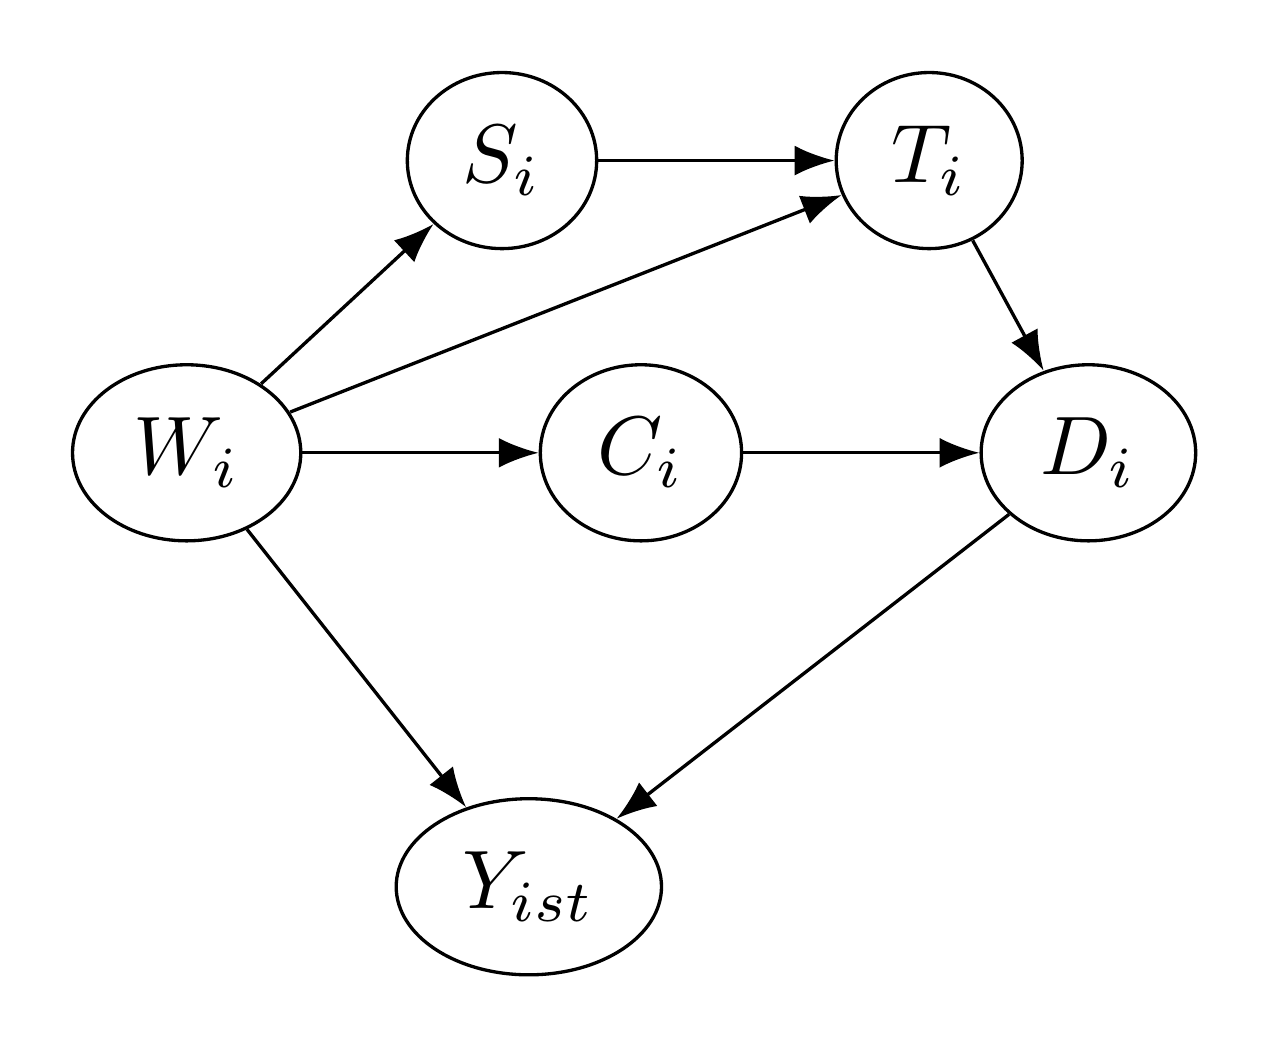
\includegraphics[width = 0.6\textwidth]{DAG2.png}
		\caption{Causal diagram indicating the conditional independence assumptions needed to estimate the PATT-C.\label{fig:DAG}}
		%\caption{\label{fig:DAG} here}
	\end{center}
\end{figure}

Interference undermines the framework because it creates more than two potential outcomes per participant, depending on the \textcolor{red}{received treatment} of other participants \citep{rubin1990}. We therefore assume no interference between units: 

\vskip 0.2in
\begin{assumption}{5}{}\label{sutva}
	The potential outcomes $Y_{isd}$ do not depend on $D_j$, $\forall j\neq i$. 
\end{assumption} 

\textcolor{red}{We also include the following assumptions made by \citet{Angrist1996} to identify the average
causal effect for compliers.} Assumption \eqref{monotonicity} ensures that crossover is only possible from treatment to control:

\vskip 0.2in
\begin{assumption}{6}{}\label{monotonicity}
No defiers: 
\begin{equation*}
T_i \geq D_i, \qquad \forall \, i \, , \, d, t=\{0,1\}.
\end{equation*}
\end{assumption}
\noindent
Assumption \eqref{ER} ensures treatment assignment affects the response only through the treatment received. In particular, the treatment effect may only be nonzero for compliers.

\begin{assumption}{7}{}\label{ER}
Exclusion restriction: For noncompliers,
\begin{equation*}
Y_{i11} = Y_{i10}, \qquad \forall \, i.
\end{equation*}  
\end{assumption}

\subsection{PATT-C}

PATT-C is interpreted as the complier-average causal effect estimated on the RCT sample extrapolated to what we would have observed in the population if treatment received $D_i$ is the same. \textcolor{red}{It is written as follows:}
%
\begin{equation}\label{tpattc}
\tau_{\text{PATT-C}} = \ex\left( Y_{i01} - Y_{i00} \mid S_i=0, D_i=1\right).
\end{equation}
%
The following theorem relates the treatment effect in the RCT to the treatment effect in the population. 

\vskip 0.2in
\begin{theorem}\label{thm1}
Under Assumptions \eqref{consistency} -- \eqref{ER},
\begin{equation}\label{tpattc-est}
\tau_{\text{PATT-C}} = \ex_{01}\left[  \ex\left(Y_{i11} \mid S_i=1, D_i=1, W_i\right)\right]
-\ex_{01}\left[  \ex\left(Y_{i10} \mid S_i=1, T_i =0, C_i =1, W_i\right) \right] 
\end{equation}

where $\ex_{01}\left[\ex(\cdot \mid\dots, W_i)\right]$ denotes the expectation with respect to the distribution of $W_i$ for population members who received treatment.
\end{theorem}

\begin{proof}
We separate the expectation linearly into two terms and consider each individually.
\begin{align*}
\ex\left(Y_{i01} \mid S_i=0,D_i=1\right) &= \ex\left(Y_{i11} \mid S_i=0, D_i=1\right) \tag*{by Assumption \eqref{consistency}} \\
&= \ex\left(Y_{i11} \mid S_i=0, T_i=1, C_i=1\right) \tag*{by Assumption \eqref{monotonicity}} \\
&= \ex_{01}\left[  \ex\left(Y_{i11} \mid S_i=0, T_i=1, C_i=1, W_i\right) \right] \\
&= \ex_{01}\left[  \ex\left(Y_{i11} \mid S_i=1, T_i=1, C_i=1, W_i\right) \right] \tag*{by Assumption \eqref{si_treat}} \\
&= \ex_{01}\left[  \ex\left(Y_{i11} \mid S_i=1, D_i=1, W_i\right)\right] 
\end{align*}

Intuitively, conditioning on $W_i$ makes sample selection ignorable under Assumption \eqref{si_treat}. This is the critical connector between the third and fourth lines of the first expectation derivation.
	
\begin{align*}
\ex\left(Y_{i00} \mid S_i=0, D_i=1\right) &= \ex\left(Y_{i10} \mid S_i=0, D_i=1\right) \tag*{by Assumption \eqref{consistency}} \\
&= \ex\left(Y_{i10} \mid S_i=0, T_i=1, C_i=1\right) \tag*{by Assumption \eqref{monotonicity}} \\
&= \ex_{01}\left[  \ex\left(Y_{i10} \mid S_i=1, T_i=1, C_i=1, W_i\right) \right] \tag*{by Assumption \eqref{si_ctrl}} \\
&= \ex_{01}\left[  \ex\left(Y_{i10} \mid S_i=1, T_i=0, C_i=1, W_i\right) \right] \tag*{by Assumption \eqref{compl}}\\
\end{align*}

The last line follows because Assumption \eqref{compl} allows us to use RCT controls who would have complied had they been assigned to treatment. Finally, the result follows by plugging these two expressions into Eq.~\eqref{tpattc}.
\end{proof}

\section{Estimation procedure}\label{estimation}

There are two challenges in turning Theorem~\eqref{thm1} into an estimator of $\tau_{\text{PATT-C}}$ in practice. First, we must estimate the inner expectation over potential outcomes of compliers in the RCT. In the empirical example, we use an ensemble of algorithms \citep{van2007} to estimate the response surface for compliers in the RCT, given their covariates. Thus, the first term in the expression for $\tau_{\text{PATT-C}}$ is estimated by the weighted average of points on the response surface, evaluated for each treated population member's potential outcome under treatment. The second term is estimated by the weighted average of points on the response surface, evaluated for each treated population member's potential outcome under control.

The second challenge is that we cannot observe which individuals are included in the estimation of the second term. In the RCT control group, $C_i$ is unobservable, as they always receive no treatment ($D_i=0$). We must estimate the second term of Eq.~\eqref{tpattc-est} by predicting who in the control group would be a complier had they been assigned to treatment. \textcolor{red}{Explicitly modeling compliance allows us to decompose PATT-C estimates by subgroup according to covariates common to both RCT and observational datasets. This approach also accounts for settings where the compliance rate differs between the sample and population, as well as across subgroups.}

The procedure for estimating $\tau_{\text{PATT-C}}$ using Theorem~\eqref{thm1} is as follows:
\begin{enumerate}[label=\textbf{S.\arabic*},ref=S.\arabic*]
\item Using the group assigned to treatment in the RCT $(S_i=1, T_i=1)$, train a model (or an ensemble of models) to predict the probability of compliance as a function of covariates $W_i$. \label{compliance-model}
\item Using the model from \ref{compliance-model}, predict who in the RCT assigned to control \textit{would have} complied to treatment had they been assigned to the treatment group.\footnote{We use a standard prediction threshold of 50\% in order classify compliers, $C_i=1$. Adjusting the prediction threshold upward would result in more accurate classifications, although we do not explore this approach.} \label{complier-predict}
\item For the observed compliers assigned to treatment and predicted compliers assigned to control, train a model to predict the response using $W_i$ and $D_i$, which gives $\ex(Y_{i1d} \mid S_i=1, D_i=d, W_i)$ for $d \in \{0,1\}$.\label{response-model}
\item For all individuals who received treatment in the population $(S_i=0, D_i=1)$, estimate their potential outcomes using the model from \ref{response-model}, which gives $Y_{i1d}$ for $d \in \{0,1\}$. The mean counterfactual $Y_{i11}$ minus the mean counterfactual $Y_{i10}$ is the estimate of $\tau_{\text{PATT-C}}$.\label{response-predict}
\end{enumerate}

Assumptions \eqref{si_treat} and \eqref{si_ctrl} are particularly important for estimating $\tau_{\text{PATT-C}}$: the success of the proposed estimator hinges on the assumption that the response surface is the same for compliers in the RCT and target population. If this does not hold, then the potential outcomes $Y_{i10}$ and $Y_{i11}$ for target population individuals cannot be estimated using the model from \ref{response-model}. Section \ref{verifying} discusses whether the strong ignorability assumptions are plausible in the empirical application.

\subsection{Modeling assumptions}  \label{modeling-assumptions}

In addition to the identification assumptions, we require additional modeling assumptions for the estimation procedure. As pointed out in Section \ref{assumptions}, we require that $W_i$ is complete because if any relevant elements of $W_i$ are not controlled, then there is a backdoor pathway from $T_i$ back to $W_i$ and into $Y_{isd}$. \textcolor{red}{Additionally,} we assume that the compliance model is accurate in predicting compliance in the training sample of RCT participants assigned to treatment and also generalizable to RCT participants assigned to control (\ref{compliance-model} and \ref{complier-predict}). Section \ref{ensemble} below describes the method of evaluating the generalizability of the compliance model.

\subsection{Ensemble method}  \label{ensemble}

In the empirical application, we use the weighted ensemble method described in \citet{van2007} for \ref{compliance-model} and \ref{response-model} of the estimation procedure. This ensemble method combines algorithms with a convex combination of weights based on minimizing cross-validated error. It is shown to control for overfitting and outperforms single algorithms selected by cross-validation \citep{polley2010super}. 

We choose a variety of candidate algorithms to construct the ensemble, with a preference towards algorithms that tend to outperform in supervised classification tasks. We also have a preference for algorithms that have a built-in variable selection property. The idea is that we input the same $W_i$ and each candidate algorithm selects the most important covariates for predicting compliance status or potential outcomes.\footnote{A potential concern when predicting potential outcomes is that the algorithm might shrink the treatment received predictor to zero, which would result in no difference between counterfactual potential outcomes.} We select three types of candidate algorithms: nonparametric additive regression models \citep{buja1989linear}; L1 or L2-regularized linear models (i.e., Lasso or ridge regression, respectively) \citep{tibshirani2012strong}; and ensembles of decision trees (i.e., random forests) \citep{breiman2001}. L1-regularized linear models are important for the application due to their variable selection properties: Lasso is particularly attractive because it tends to shrink all but one of the coefficients of correlated covariates to zero. 

\section{Simulations} \label{sim}

We conduct a simulation study comparing the performance of the \textcolor{red}{PATT-C estimator against its unadjusted analogue, which we refer to as the Population Average Treatment Effect on the Treated (PATT):
%	
\begin{equation}\label{tpatt}
\tau_{\text{PATT}} = \ex\left( Y_{i01} - Y_{i00} \mid S_i=0, D_i=1\right).
\end{equation}
%
Eq.~\eqref{tpatt} identifies the population-average causal effect of taking up treatment, adjusted according to the covariate distribution of population members who received treatment. We estimate the response curve for all RCT participants, conditional on their covariates and actual treatment received. Identical to \ref{response-predict} in the estimation procedure for PATT-C, we use the response model to estimate the outcomes of population members who received treatment given their covariates, which are then used to estimate Eq.~\eqref{tpatt}. Like the PATT-C estimator, the PATT estimator crucially relies on the assumption that the response surface is the same for RCT participants and population members who received treatment.}

\textcolor{red}{
We compare the population estimators against the sample Complier Average Causal Effect (CACE) \citep{imbens1997bayesian}, which is commonly referred to the Local Average Treatment Effect in the econometrics literature \citep{imbens1994identification,Angrist1996}. In the context of program evaluation, it is a more relevant treatment effect of interest than the ITT effect because only RCT participants who received treatment would have their outcomes affected by treatment in the presence of a nonnegative treatment effect.} 

\textcolor{red}{
CACE is defined as the average causal effect of treatment received restricted to sample compliers:
%	
\begin{equation}\label{tcace}
\tau_{\text{CACE}} = \ex\left( Y_{i11} - Y_{i10} \mid S_i=1, C_i=1\right).
\end{equation}	
%
In other words, CACE is the treatment effect for RCT participants who would comply regardless of treatment assignment. However, we are unable to observe the compliance status of RCT participants assigned to control because we do not know if they would have complied if they had been assigned to treatment. A generalization of the instrumental variables estimator of the CACE in the presence of noncompliers is given by:
%	
\begin{equation}\label{tcace-hat}
\hat{\tau}_{\text{CACE}} = \frac{\ex\left( Y_{i11} - Y_{i10} \mid S_i=1\right)}{\pr(T_i = D_i = 1 \mid S_i=1)},
\end{equation}	
%
which is equivalent to scaling the ITT effect by the sample proportion of treated compliers \citep[e.g.,][]{freedman2006}. Eq.~\eqref{tcace-hat} is identified under Assumptions \eqref{sutva}, \eqref{monotonicity}, and \eqref{ER}.}

\subsection{Simulation design}

The simulation is designed so that the effect of treatment is heterogeneous and depends on covariates which are different in the RCT and target population. The design satisfies the conditional independence assumptions in Figure~\ref{fig:DAG}.

In the simulation, RCT eligibility, complier status, and treatment assignment in the population depend on multivariate normal covariates $(W^{1}_i, W^{2}_i, W^{3}_i, W^{4}_i)$ with means $(0.5, 1, -1, -1)$ and covariances $\cov(W^{1}_i, W^{2}_i) = \cov(W^{1}_i, W^{4}_i)= \cov(W^{2}_i, W^{4}_i) = \cov(W^{3}_i, W^{4}_i) = 1$ and $\cov(W^{1}_i, W^{3}_i) = \cov(W^{2}_i, W^{3}_i) = 0.5$.  The first three covariates are observed by the researcher and $W^{4}_i$ is unobserved. \textcolor{red}{$U_i, V_i, R_i$, and $Q_i$ are standard normal error terms. $U_i, V_i, R_i, Q_i$, and $(W^{1}_i, W^{2}_i, W^{3}_i, W^{4}_i)$ are mutually independent.} 

The equation for selection into the RCT is
%	
\begin{equation*}
S_i = \ind(e_2 + g_1W^{1}_i + g_2W^{2}_i + g_3W^{3}_i + e_4W^{4}_i + R_i > 0).
\end{equation*}	
%
The parameter $e_2$ varies the fraction of the population eligible for the RCT and $e_4$ varies the degree of confounding with sample selection. We set the constants $g_1, g_2,$ and $g_3$ to be $0.5,$ $0.25,$ and $0.75$, respectively. 

Complier status is determined by
%	
\begin{equation*}
C_i = \ind(e_3 + h_2W^{2}_i + h_3W^{3}_i + e_5W^{4}_i + Q_i > 0),
\end{equation*}	
%
where $e_3$ varies the fraction of compliers in the population, and $e_5$ varies the degree of confounding with treatment assignment. We set the constants $h_2$ and $h_3$ to $0.5$. 

For individuals in the population ($S_i=0$), treatment is assigned by
%	
\begin{equation*}
T_i = \ind(e_1 + f_1W^{1}_i + f_2W^{2}_i + e_6W^{4}_i + V_i > 0),
\end{equation*}	
%
where $e_1$ varies the fraction eligible for treatment in the population and $e_6$ varies the degree of confounding with sample selection. We set the constants $f_1$ and $f_2$ to $0.25$ and $0.75$, respectively. For individuals in the RCT ($S_1=1$), treatment assignment \textcolor{red}{$T_i$} is a sample from a Bernoulli distribution with probability $p=0.5$.

Finally, the response is determined by 
%	
\begin{align*}
Y_{isd} &= a + bD_i + c_1W^{1}_i + c_2W^{2}_i + \textcolor{red}{c_3W^{4}} +dU_i,
\end{align*}
%
where we set $a, c_1, \textcolor{red}{c_3,}$ and $d$ to $1$ and $c_2$ to $2$. The treatment effect $b$ is heterogeneous:
\begin{align*}
b &= \left\{
			\begin{array}{rr}
        1, & \text{if } W^{1}_i > 0.75\\
		-1, & \text{if } W^{1}_i \leq 0.75\\
			\end{array}\right.
\end{align*}	 
 
We generate a population of 30,000 individuals and randomly sample 5,000. Those among the 5,000 who are eligible for the RCT ($S_i=1$) are selected. Similarly, we sample 5,000 individuals from the population and select those who are not eligible for the RCT ($S_i=0$) \textcolor{red}{to be our} observational study participants.\footnote{This set-up mimics the reality that a population census is usually impossible.} We set each individual's treatment received $D_i$ according to their treatment assignment and complier status and observe their responses $Y_{isd}$. In this design, the manner in which $S_i$, $T_i$, $D_i$, $C_i$, and $Y_{isd}$ are simulated ensures that Assumptions \eqref{consistency} -- \eqref{ER} hold.

In the assigned-treatment RCT group $(S_i = 1, T_i = 1)$, we train a gradient boosting algorithm \citep{friedman2001greedy} on the covariates to predict who in the control group $(S_i = 1, T_i = 0)$ would comply with treatment ($C_i=1$), which is unobservable. These individuals \textit{would have} complied had they been assigned to the treatment group. For this group of observed compliers to treatment and predicted compliers from the control group of the RCT, we estimate the response surface using gradient boosting with features $(W^{1}_i, W^{2}_i, W^{3}_i)$ and $D_i$. The PATT-C is estimated according to the estimation procedure outlined above.

\subsection{Simulation results}\label{sim-results}

We vary each of the parameters $e_1$, $e_2$, $e_3$, $e_4$, $e_5$, and $e_6$ along a grid of five random standard normal values in order to generate different combinations of rates of compliance, treatment eligibility, RCT eligibility in the population, and confounding. For each possible combination of the six parameters, \textcolor{red}{and holding all other parameters constant, we compute over 10 simulation runs the average root mean squared error (RMSE) between the true population average treatment effect and the PATT-C, PATT, or CACE estimates. Averaging across combinations, the unadjusted population estimator yields the highest average RMSE (1.06), followed by the CACE (0.89), and the PATT-C (0.76).} 

\textcolor{red}{Figures~\ref{fig:rmse_ratec_rates} and \ref{fig:rmse_ratec_ratet} show the average RMSE of the estimators as a function of the population compliance rate and the share of population members eligible to participate in the RCT or the population treatment rate, respectively. The PATT estimator does not correct for bias resulting from noncompliance in the population and consequently performs poorly when the population compliance rate is relatively low (i.e., $\leq 60\%$). The PATT-C estimator corrects for noncompliance in the population and thus outperforms the PATT in low-compliance settings. The CACE corrects for noncompliance in the sample, and underperforms compared to the PATT-C due to differences between the sample and population.}

\begin{figure}[htbp]
	\begin{center}
		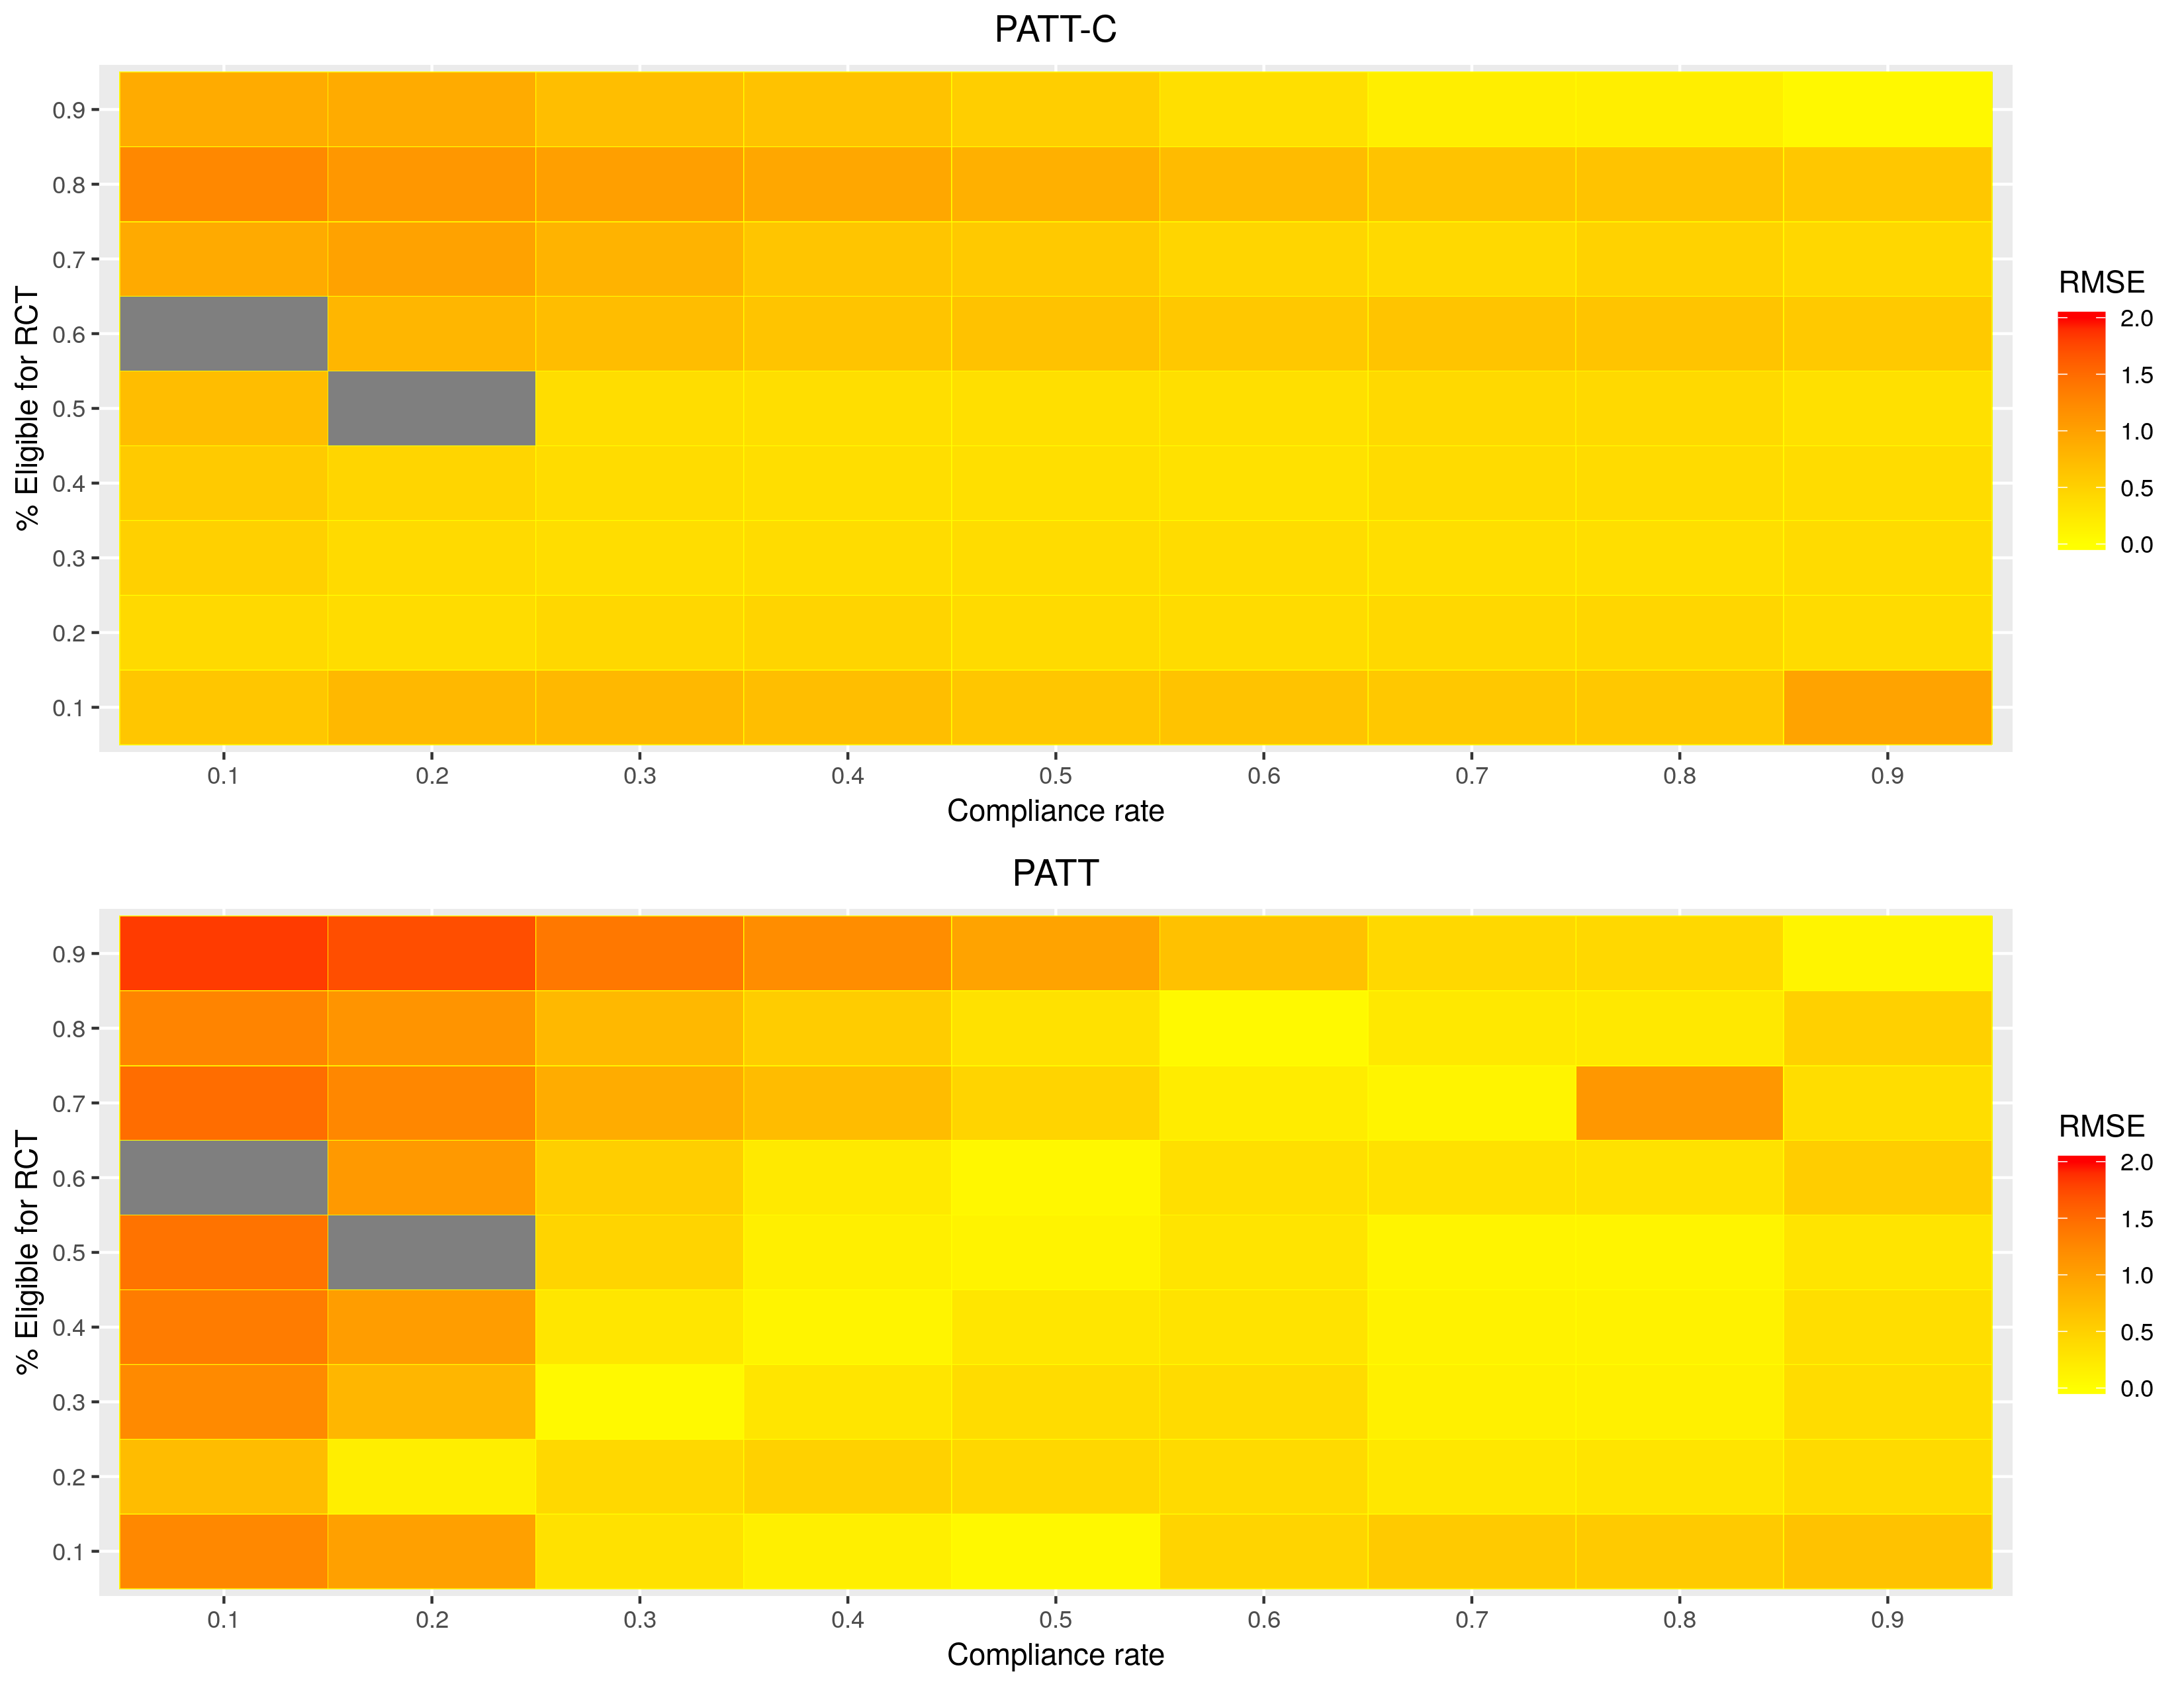
\includegraphics[width = 1\textwidth]{rmse_ratec_rates.png}
		\caption{Average RMSE, binned by compliance rate and percent eligible for the RCT. Darker tiles correspond to higher errors and white tiles correspond to missing simulated data.\label{fig:rmse_ratec_rates}}
%		\caption{\label{fig:rmse_ratec_rates} here}
	\end{center}
\end{figure}

\textcolor{red}{Figure~\ref{fig:rmse_boxplots_rateC} compares the average RMSE of the estimators at varying levels of compliance in the population. The error for each of the estimators predictably decreases as a greater share of population members comply with treatment. PATT-C outperforms both PATT and CACE in terms of minimizing RMSE when the population compliance rate is below 90\%. The PATT outperforms the PATT-C only at nearly perfect population compliance (i.e., 90\% compliance rate), and the CACE outperforms the PATT when the population compliance rate is at 60\% or below.} 

\textcolor{red}{Figures~\ref{fig:rmse_boxplots_RateConC}, \ref{fig:rmse_boxplots_RateConT}, and \ref{fig:rmse_boxplots_RateConS} plot the relationships between estimation error and the degrees of confounding in the mechanisms that determine compliance, treatment assignment, and sample selection, respectively. The estimation error of PATT-C is comparatively less invariant to increases in the degree of confounding in the three mechanisms compared to its unadjusted counterpart. The estimation error of CACE is generally more variable than that of the population estimators due to CACE's inability to account for differences between the sample and target population.}

\begin{figure}[htbp]
\begin{center}
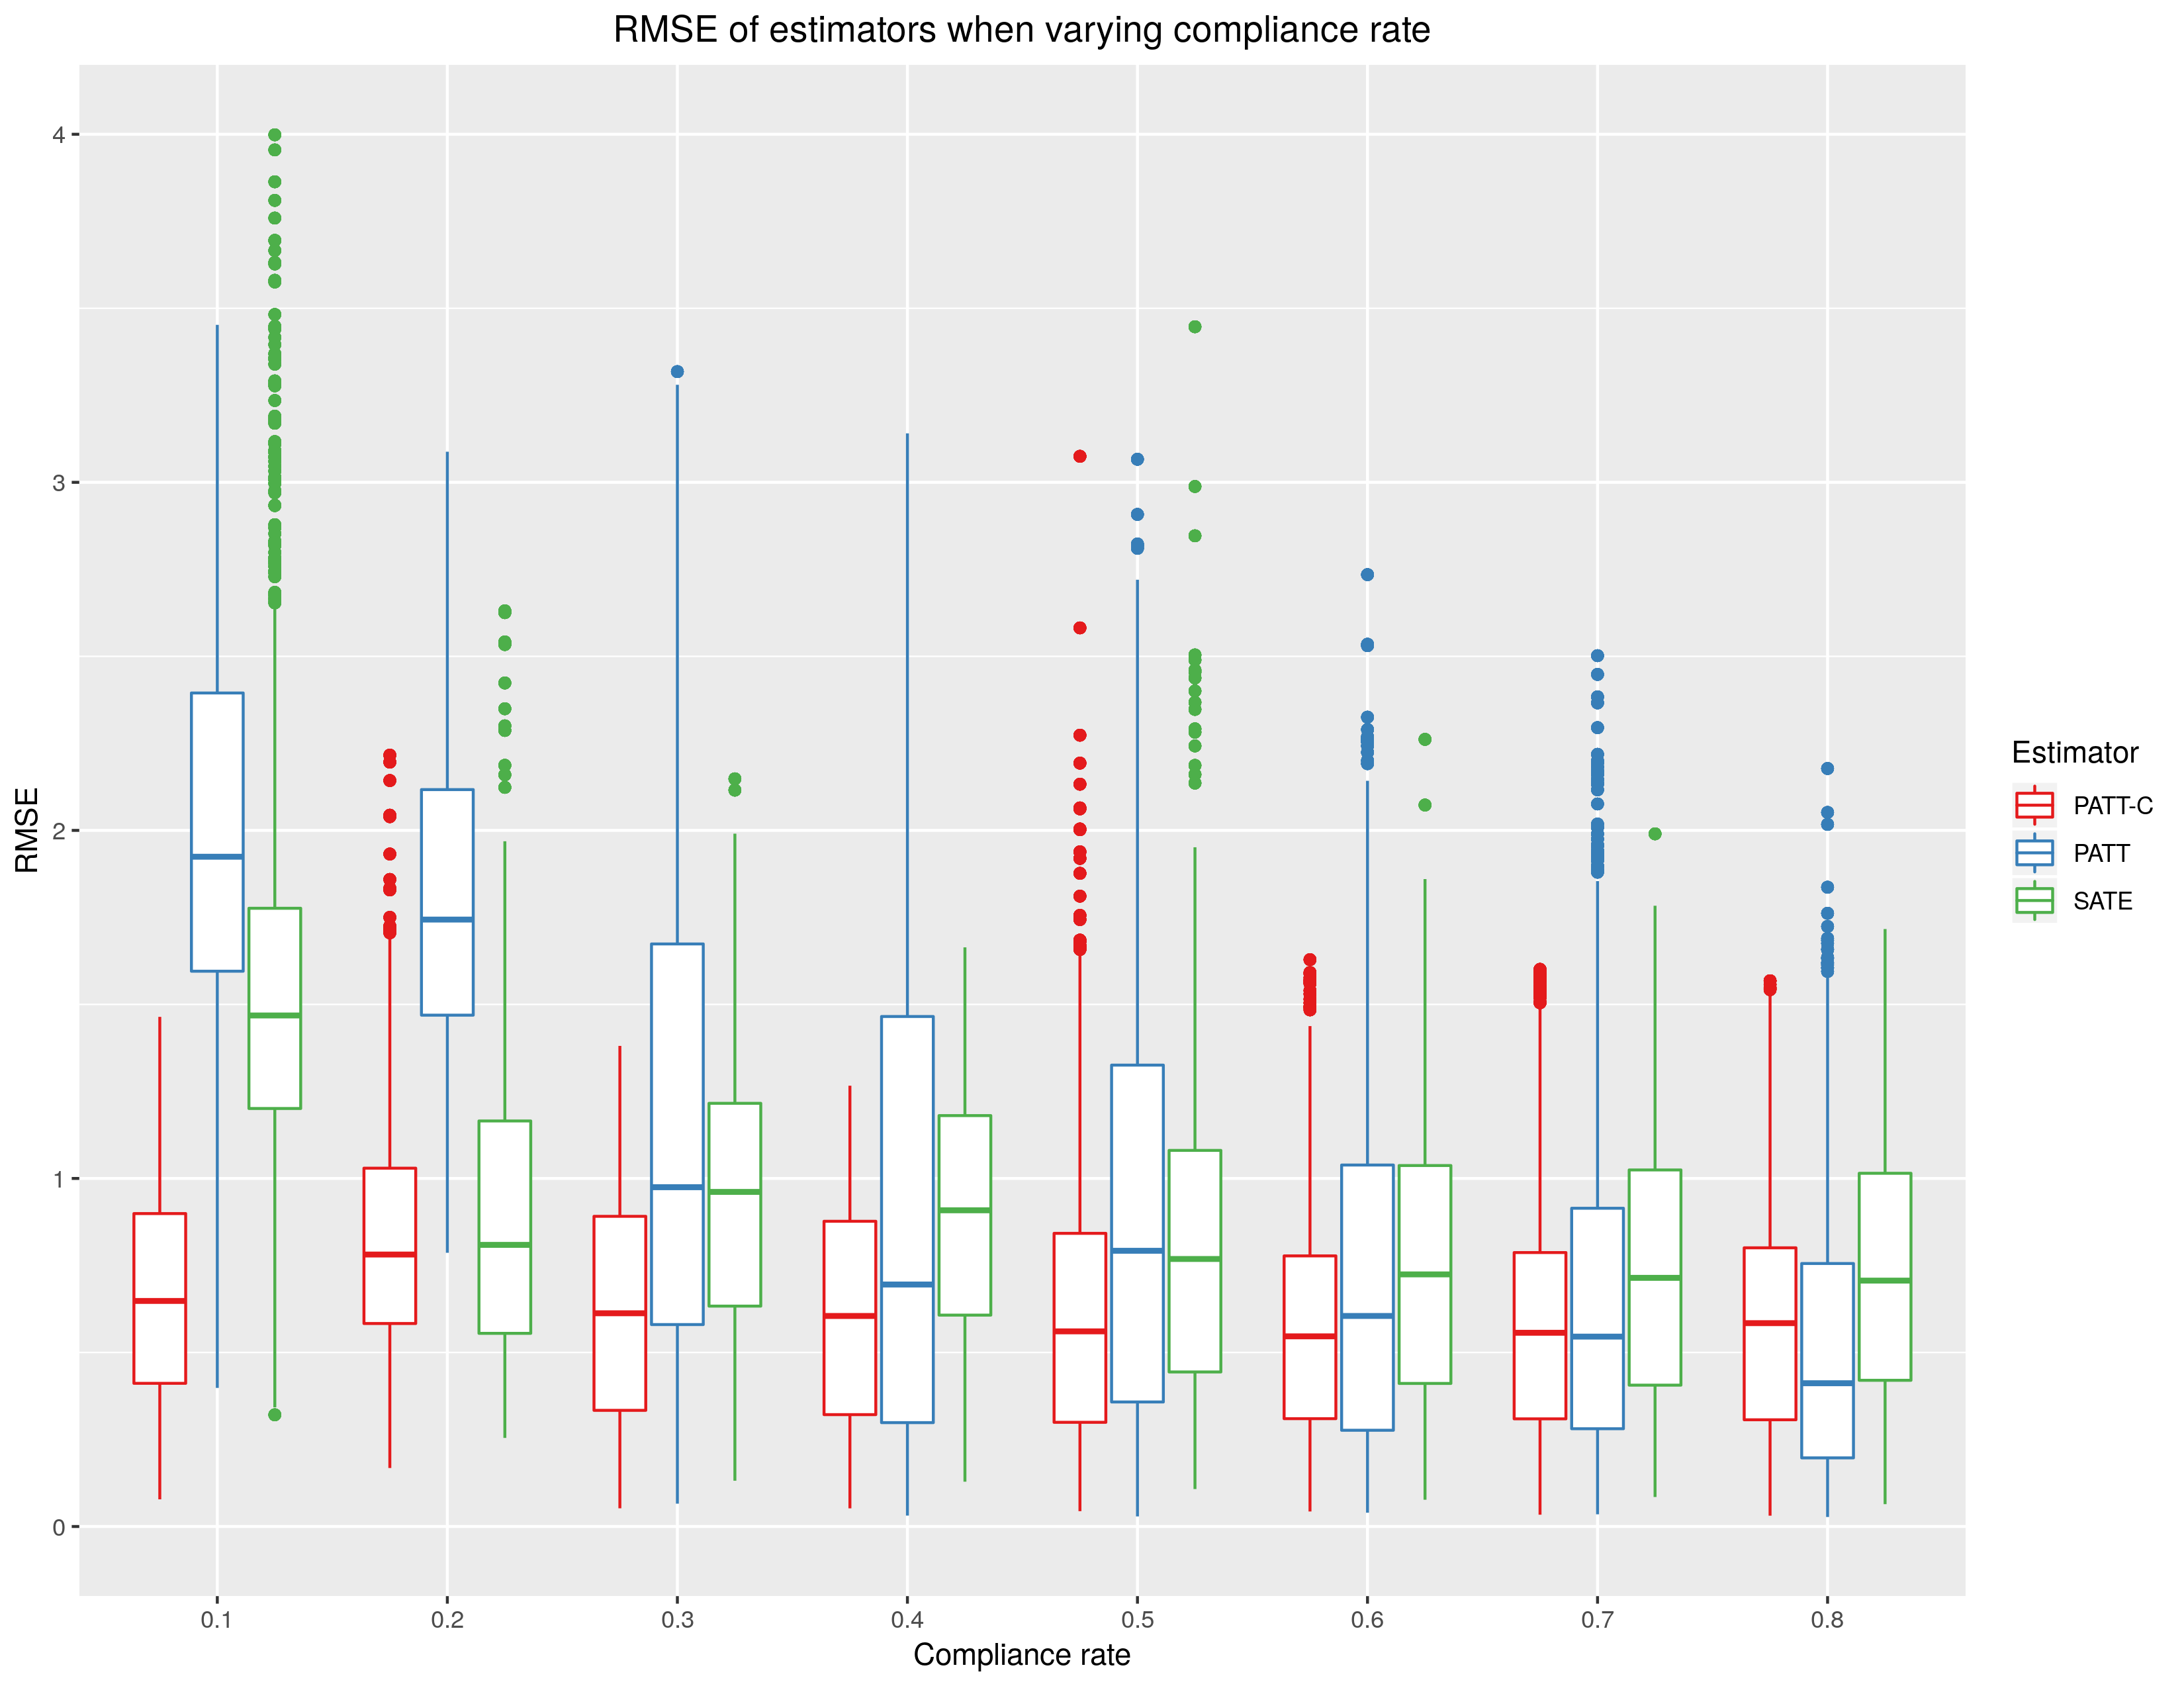
\includegraphics[width = 1\textwidth]{rmse_boxplots_rateC.png}
\caption{Average RMSE according to compliance rates in the population.\label{fig:rmse_boxplots_rateC}}
%\caption{\label{fig:rmse_boxplots_rateC} here}
\end{center}
\end{figure}

\pagebreak
\section{Application: Medicaid and health care use} \label{application}

We apply the proposed estimator to measure the effect of Medicaid coverage on health care use for a target population of adults who may benefit from expansions to the Medicaid program. In particular, we examine the population of nonelderly adults in the U.S. with household incomes at or below 138\% of the Federal Poverty Level (FPL) --- which amounts to \$32,913 for a four--person household in 2014 --- who may be eligible for Medicaid following the Affordable Care Act (ACA) expansion.

We draw RCT data from the Oregon Health Insurance Experiment (OHIE) \citep{finkelstein2012,Taubman}, \textcolor{red}{which randomly assigned Medicaid coverage to the uninsured and examined their subsequent health care use.} Subsequent research calls in to question the external validity of the OHIE, which resulted in the counterintuitive finding that Medicaid increased ER use among RCT participants. For example, quasi-experimental studies on the impact of the 2006 Massachusetts health reform --- which served as a model for the ACA --- show that ER use decreased or remained constant following the reform \citep{miller2012effect, kolstad2012impact}. A challenge to the external validity of the OHIE is that it's exclusion criteria was likely more restrictive than government health insurance expansions. 

\subsection{RCT sample} 

In 2008, \textcolor{red}{a group of uninsured low-income adults participated in the OHIE for the chance to apply to receive health insurance through a state Medicaid program. In line with program eligibility requirements, participants were restricted to Oregon residents aged 19 to 64 who were not otherwise eligible for public insurance, who had been without insurance for six months, had income below the FPL, and held assets below \$2,000.} Treatment \textcolor{red}{assignment} occurred at the household level: participants selected by the lottery won the opportunity for themselves and any household member to apply for Medicaid. Within a sample of 74,922 individuals representing 66,385 households, 29,834 participants were selected by the lottery; the remaining 45,008 participants served as controls in the experiment. 

Participants in selected households \textcolor{red}{were enrolled in Medicaid} if they returned an enrollment application within 45 days of receipt. \textcolor{red}{Only 30\% of participants in selected households successfully enrolled. The low compliance rate is primarily due to failure to return an application or demonstrate income below the FPL. Compliance is measured using a binary variable indicating whether the participant was enrolled in any Medicaid program during the study period.}

\textcolor{red}{We include as covariates in our response and complier models (\ref{compliance-model} and \ref{response-model}, respectively) pretreatment information on participant age, race, gender, education, marital status, number of children in the household, employment status, health status, and household income. We also include indicator variables on household size because lottery selection was random conditional on the number of household members. Because treatment occurs at the household level, all analyses cluster standard errors at the household level.} 

The response data originate from a mail survey \textcolor{red}{containing questions about health insurance and health care use that elicited responses from 23,741 OHIE participants.\footnote{Following \citet{finkelstein2012}, indicator variables for survey wave and interactions with household size indicators are also included as covariates in the response and complier models because the proportion of treated participants varies across the survey waves.} The response variables measure health care use in terms of the number of ER and primary care (i.e., outpatient) visits in the past six months}. 

\subsection{Observational data} 

We acquire data on the target population from the National Health Interview Study (NHIS) for years 2008 to 2017.\footnote{A possible limitation of this application is that it ignores the complex sampling techniques of the NHIS sample design such as differential sampling, which is discussed in detail in \citet{parsons2014design}.} We restrict the sample to respondents with income below 138\% of the FPL and who are uninsured or on Medicaid and select covariates on respondent characteristics that match the OHIE pretreatment covariates. We use a recoded variable that indicates whether respondents are on Medicaid as an analogue to the OHIE compliance measure. \textcolor{red}{The outcomes of interest from the NHIS are based on questions that are virtually identical to the OHIE mail survey questions, except that the utilization questions in the NHIS are asked with a 12 month rather than a 6 month look-back period.\footnote{Following \citet{finkelstein2012}, we resolve this discrepancy by halving the NHIS responses in order to make them comparable to the OHIE outcomes.}}

\subsection{Verifying assumptions} \label{verifying}

In order for $\tau_{\text{PATT-C}}$ to be identified, Assumptions \eqref{consistency} -- \eqref{ER} must be met. Assumption \eqref{consistency} ensures that potential outcomes for participants in the target population would be identical to their outcomes in the RCT if they had been randomly assigned their observed treatment. In the empirical application, Medicaid coverage for uninsured individuals was applied in the same manner in the RCT as it is in the population.  Differences in potential outcomes due to sample selection might arise, however, if there are differences in the mail surveys used to elicit health care use responses between the RCT and the nonrandomized study. 

We cannot directly test Assumptions \eqref{si_treat} and \eqref{si_ctrl}, which state that potential outcomes for treatment and control are independent of sample assignment for individuals with the same covariates and assignment to treatment. The assumptions are only met if every possible confounder associated with the response and the sample assignment is accounted for. In estimating the response surface, we use all demographic, socioeconomic, and pre-existing health condition data that were common in the OHIE and NHIS data. Potentially important unobserved confounders include the number of hospital and outpatient visits in the previous year, proximity to health services, and enrollment in other federal programs. 

The final two columns of Table~\ref{rct-nrt-compare} compares RCT participants selected for Medicaid with population members on Medicaid. Compared to the RCT compliers, the \textcolor{red}{population members who received treatment} are predominantly female, younger, more racially and ethnically diverse, less educated, and live in higher income households. Diagnoses of diabetes, asthma, high blood pressure, and heart disease are more common among the population on Medicaid then the RCT treated. \textcolor{red}{These summary statistics and the analyses that follow use survey weights to account for the probability of being sampled and non-response.}

Strong ignorability assumptions may also be violated due to the fact that the OHIE applied a more stringent exclusion criteria compared to the NHIS sample. While the RCT and population sample both screened for individuals below the FPL,  \textcolor{red}{only the RCT required those enrolled to recertify their household income eligibility during the study period. Strong ignorability would not hold if the failure to recertify is correlated with unobserved variables.} 

\textcolor{red}{Following Assumption \ref{sutva}, we assume no interference between households in the OHIE because treatment assignment occured at the household level. Within-household interference is not possible in this RCT because household members share the same treatment status. Interference between households would threaten the no-interference assumption in the unlikely case that the Medicaid coverage of individuals in treated households affects the health care use of individuals in households assigned to control.} 

Assumption \eqref{compl} is violated if assignment to treatment influences the compliance status of individuals with the same covariates. The compliance ensemble can accurately classify compliance status for 77\% of treated RCT participants with only the covariates --- and not treatment assignment --- as model inputs.\footnote{The compliance ensemble is evaluated in terms of 10--fold cross--validated MSE. The distribution of MSE for the ensemble and its candidate algorithms are provided in Table \ref{compliance-ensemble}.}  This gives evidence in favor of the conditional independence assumption.

The exclusion restriction assumption \eqref{ER} ensures treatment assignment affects the response only through enrollment in Medicaid. It is reasonable that a person's enrollment in Medicaid, not just their eligibility to enroll, would affect their hospital use. For private health insurance one might argue that eligibility may be be negatively correlated with hospital use, as people with pre-existing conditions are less often eligible yet go to the hospital more frequently. This should not be the case with a federally funded program such as Medicaid. 

\subsubsection{Placebo tests} \label{placebo-tests}

Similar to the procedure proposed by \citep{Hartman}, we conduct placebo tests to check whether the average outcomes differ between the RCT compliers on Medicaid and the adjusted \textcolor{red}{population members who received Medicaid}.\footnote{Note that a placebo test for Assumption \eqref{compl} is not possible because we never observe whether RCT controls would actually take-up treatment if assigned.} If the placebo tests detect a significant difference between the mean outcomes of these groups, it would indicate that either Assumption \eqref{consistency} (for $d=1$), or Assumptions \eqref{si_treat} and \eqref{si_ctrl} are violated. 

Table \ref{placebo} reports the results of placebo tests, comparing the mean outcomes of RCT compliers against the mean outcomes of adjusted \textcolor{red}{population members who received treatment}. The former quantity is calculated from the observed RCT sample and the latter quantity is the mean counterfactual $Y_{i11}$ estimated from \ref{response-predict} of the estimation procedure.

Tests of equivalence between the two groups indicate that the differences across each outcome are not statistically significant. These results imply that the PATT-C estimator is not biased by differences in how Medicaid is delivered or health outcomes are measured between the RCT and population, or by differences in sample or population members' unobserved characteristics. 

\subsubsection{Sensitivity to no defiers assumption} \label{sens-defiers}

\citet{Angrist1996} show that the bias due to violations of Assumption \eqref{monotonicity} is equivalent to the difference of average causal effects of treatment received for compliers and defiers, multiplied by the relative proportion of defiers, 
$\pr(i\text{ is a defier}) / (\pr(i\text{ is a complier]}) - \pr(i\text{ is a defier})).$

Table \ref{ohie-status} reports the distribution of participants in the OHIE by status of treatment assignment and treatment received. Assumption \eqref{monotonicity} does not hold due to the presence of defiers; i.e., participants who were assigned to control and enrolled in Medicaid during the study period. About 6.7\% of the RCT sample were assigned to control but were enrolled in Medicaid ($T_i < D_i$) and 65.5\% of the sample complied with treatment assignment ($D_i = T_i$), which results in a bias multiplier of 0.11. Suppose that the difference of average causal effects of Medicaid received on ER use for compliers and defiers is 1.2\%. The resulting bias is only 0.1\%, which would not meaningfully alter the interpretation of the CACE or PATT-C estimates reported below. 
 
\subsection{Empirical results}\label{results}

We compare PATT-C and PATT estimates for ER and outpatient use. We obtain estimates for the overall group of participants and subgroups according to sex, age, race, health status, education, and household income. Subgroup treatment effects are estimated by taking differences across response surfaces for a given covariate subgroup, and response surfaces are estimated with the ensemble mean predictions. We use treatment received, number of household members, and the subgroup covariates as features in the response models. We generate 95\% confidence intervals for these estimates using 1,000 bootstrap samples. 

Table \ref{compliance-compare} presents the PATT-C estimates, which indicate that Medicaid coverage has a positive, but considerably smaller effect on the number of ER and outpatient visits. For comparison, \citet{finkelstein2012} reports population estimates of the effect of Medicaid coverage on the number of ER and out-patient visits using 2004--2009 NHIS data on adults aged 19--64 below 100 percent of the federal poverty line ($n=15,528$). \citet{finkelstein2012} estimates Medicaid coverage significantly increases the number of ER visits by 0.08 [0.05, 0.12] and increases the number of outpatient visits by 1.45 [1.33, 1.57]. 

Figures \ref{fig:any-visit-plot}, \ref{fig:num-visit-plot}, and \ref{fig:num-out-plot} examine heterogeneous treatment effect estimates on ER and outpatient use in the population. While this study is the first to our knowledge to estimate heterogeniety in treatment effects for the target population, \citet{Taubman} and \citet{NBERw22363} perform subgroup analyses on the RCT sample. Similar to the PATT-C estimates, \possessivecite{Taubman} subgroup analyses indicate that increases in ER use due to Medicaid are significantly larger for younger individuals and those with high school-level education.\footnote{\citet{NBERw22363} perform subgroup analyses on OHIE sample data and find larger increases in ER use as a result of Medicaid for men, English speakers, and individuals enrolled in a food stamp program prior to the lottery.}

\section{Discussion} \label{discussion}

The simulation results presented in Section \ref{sim} show that the PATT-C estimator outperforms its unadjusted counterpart when the compliance rate is low. Of course, the simulation results depend on the particular way we parameterized the compliance, selection, treatment assignment, and response schedules. 

In particular, the strength of correlation between the covariates and compliance governs how well the estimator will perform, since \ref{compliance-model} of the estimation procedure is to predict who \textit{would be} a complier in the RCT control group, had they been assigned to treatment. If it is difficult to predict compliance using the observed covariates, then the estimator will perform badly because of noise introduced by incorrectly treating noncompliers as compliers. Further research should be done into ways to test how well the model of compliance works in the population or explore models to more accurately predict compliance in RCTs.  Accurately predicting compliance is not only essential for yielding unbiased estimates of the average causal effects for target populations, it is also useful for researchers and policymakers to know which groups of individuals are unlikely to comply with treatment. 

In the OHIE trial, only about $30\%$ of those selected to receive Medicaid benefits actually enrolled. The compliance ensemble accurately classified compliance status for 77\% of treated RCT participants using only the pretreatment covariates as features. While we don't know how well the compliance ensemble predicts for the control group, the control group should be similar to the treatment group on pretreatment covariates because of the RCT randomization. The model's performance on the training set suggests that compliance is not purely random and depends on observed covariates. This gives evidence in favor of using the proposed estimator. 

In the empirical application, the sample population differs in several dimensions from the target population of individuals who will be covered by other Medicaid expansions, such as the ACA expansion to cover all adults up to 138\% of the FPL. For instance, the RCT participants are disproportionately white urban--dwellers \citep{Taubman}. The RCT participants volunteered for the study and therefore may be in poorer health compared to the target population. These differences in baseline covariates make reweighting or response surface methods necessary to extend the RCT results to the population.

Explicitly modeling compliance allows us to decompose population estimates by subgroup according to pretreatment covariates common to both RCT and observational datasets; e.g, demographic variables, pre--existing conditions, and insurance coverage. We find substantial differences between sample and population estimates in terms of race, education, and health status subgroups. This pattern is expected because RCT participants volunteered for the study and are predominately white and educated.

\pagebreak

%Bibliography
\bibliographystyle{chicago}
\bibliography{refs}

%Appendix
\pagebreak
\begin{appendices}
	
% Appendix numbering
\newcommand{\hbAppendixPrefix}{A}
%
\renewcommand{\thefigure}{\hbAppendixPrefix\arabic{figure}}
\setcounter{figure}{0}
\renewcommand{\thetable}{\hbAppendixPrefix\arabic{table}} 
\setcounter{table}{0}
\renewcommand{\theequation}{\hbAppendixPrefix\arabic{equation}} 
\setcounter{equation}{0}


\begin{figure}[htbp]
	\begin{center}
		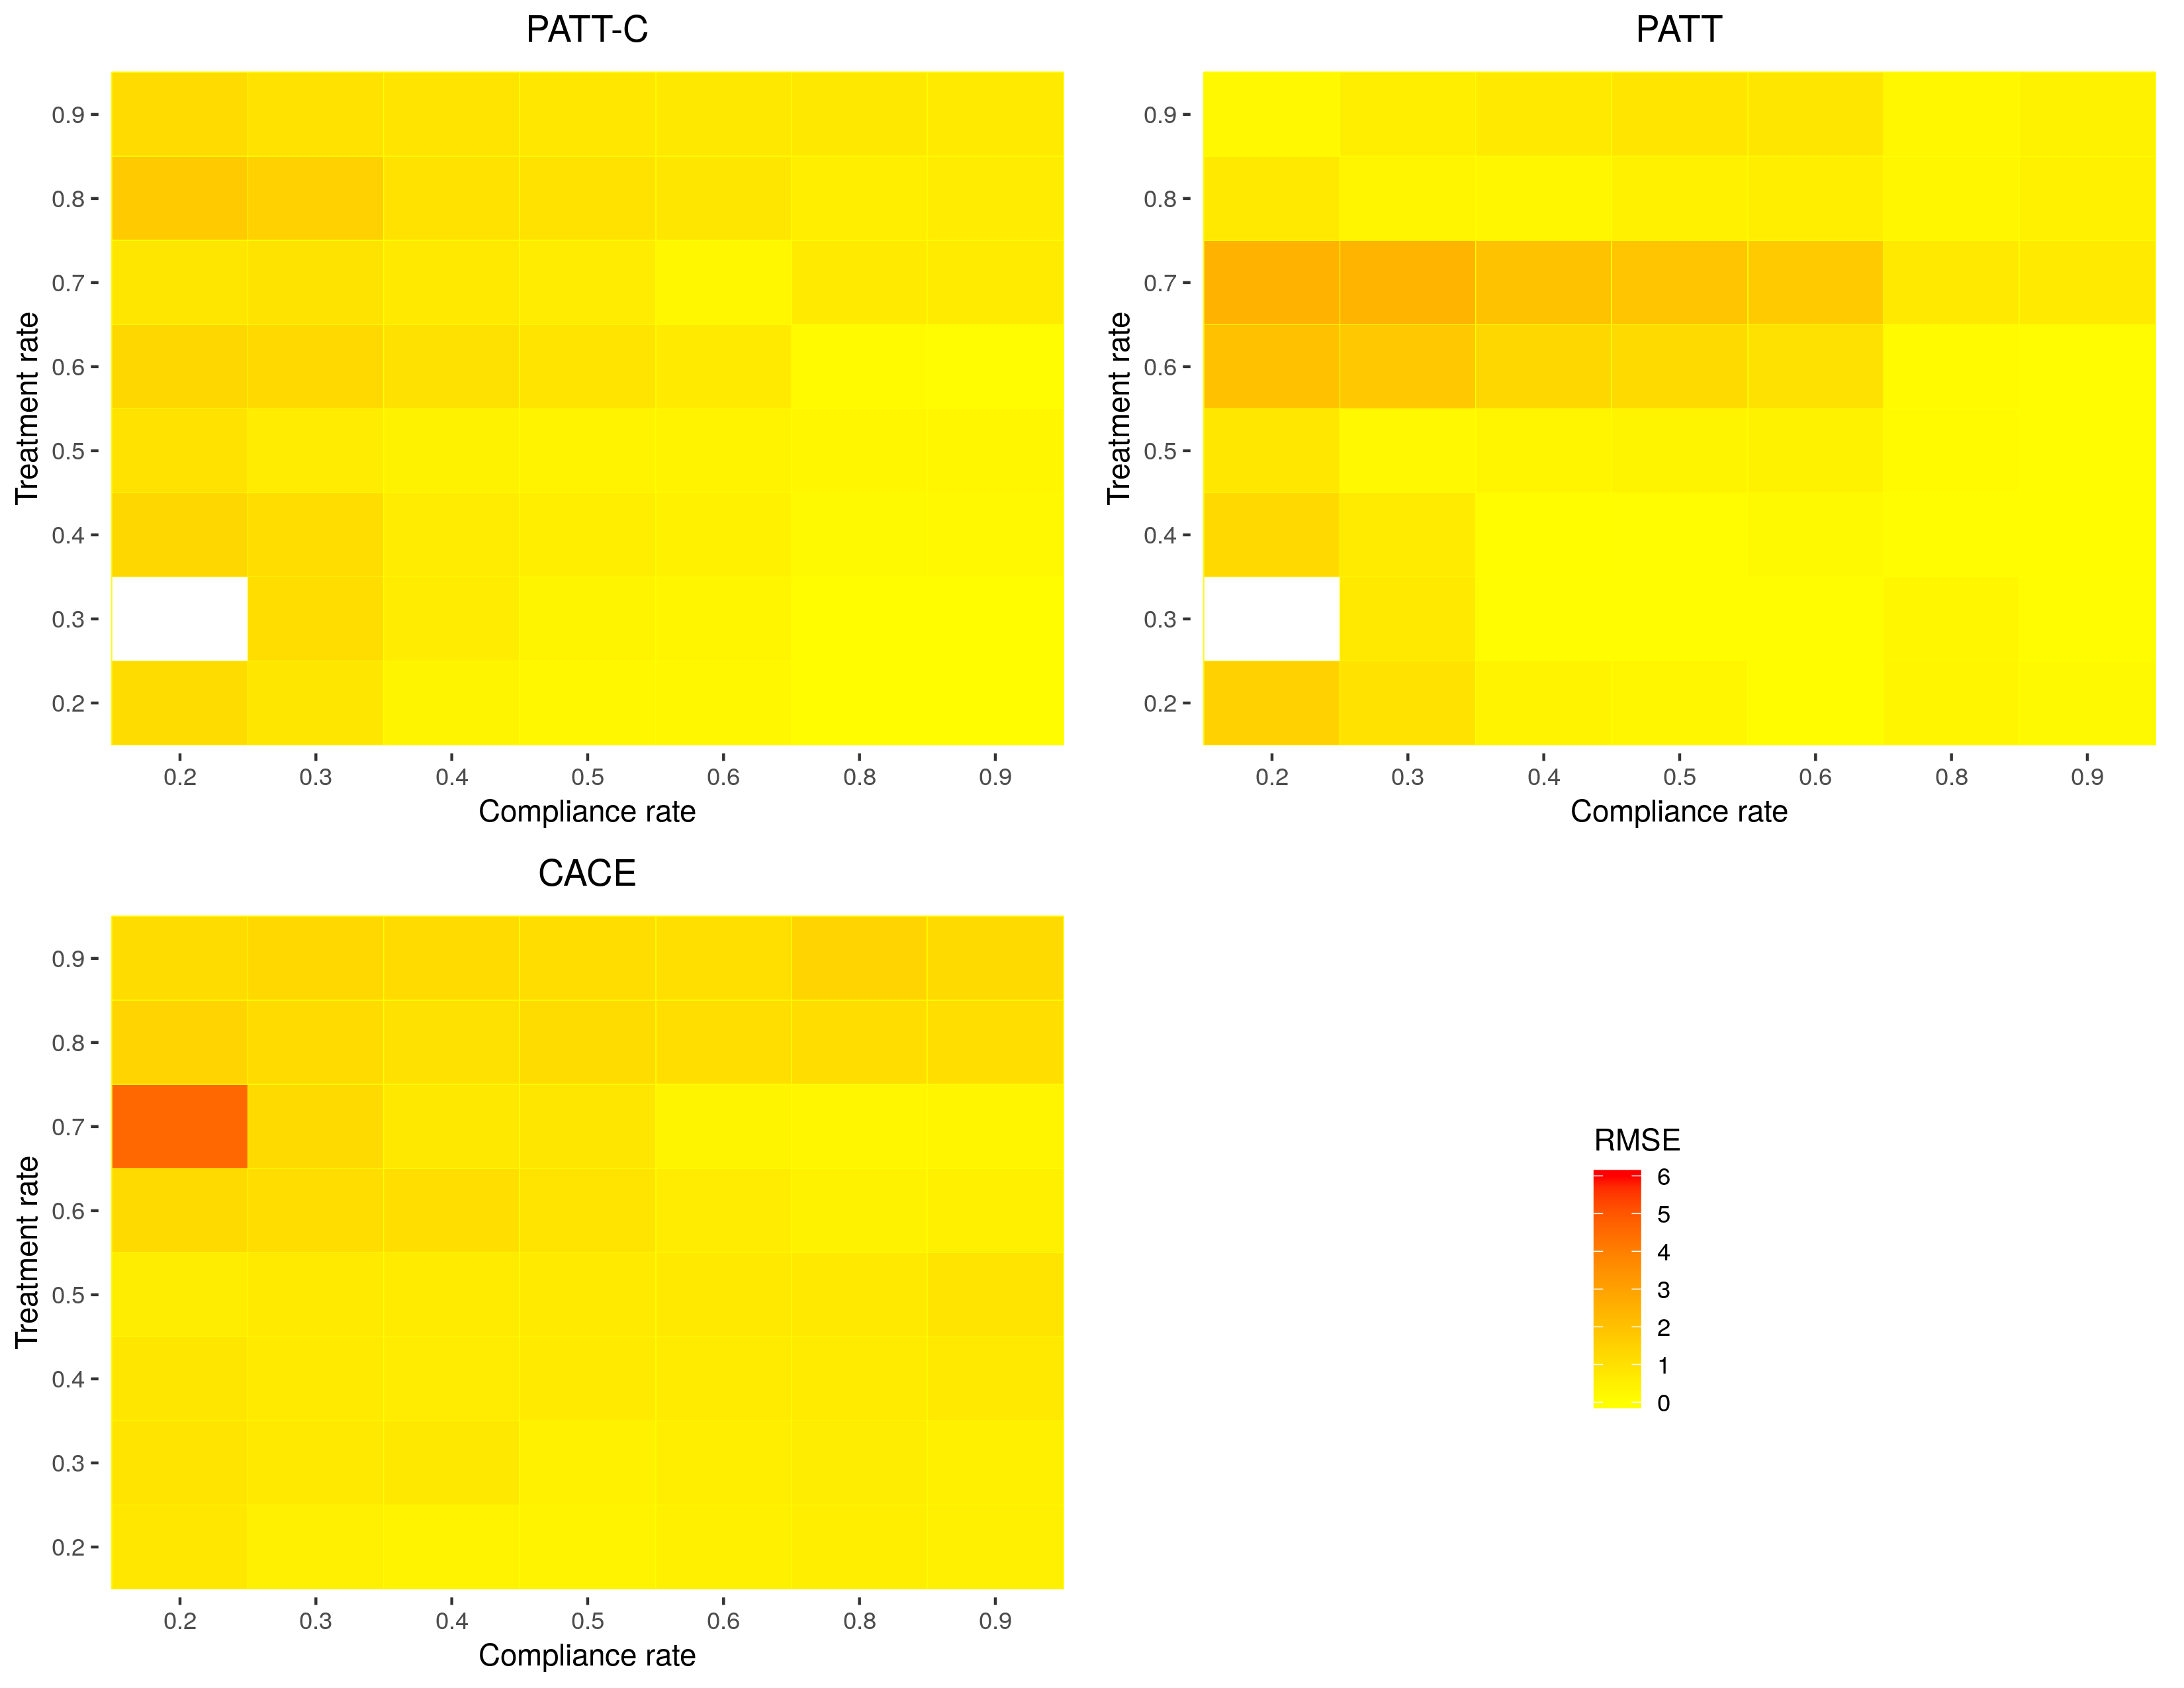
\includegraphics[width = 1\textwidth]{rmse_ratec_ratet.png}
		\caption{Average RMSE binned by compliance rate and treatment rate.\label{fig:rmse_ratec_ratet}}
%		\caption{\label{fig:rmse_ratec_ratet} here}
	\end{center}
\end{figure}

\begin{figure}[htbp]
	\begin{center}
		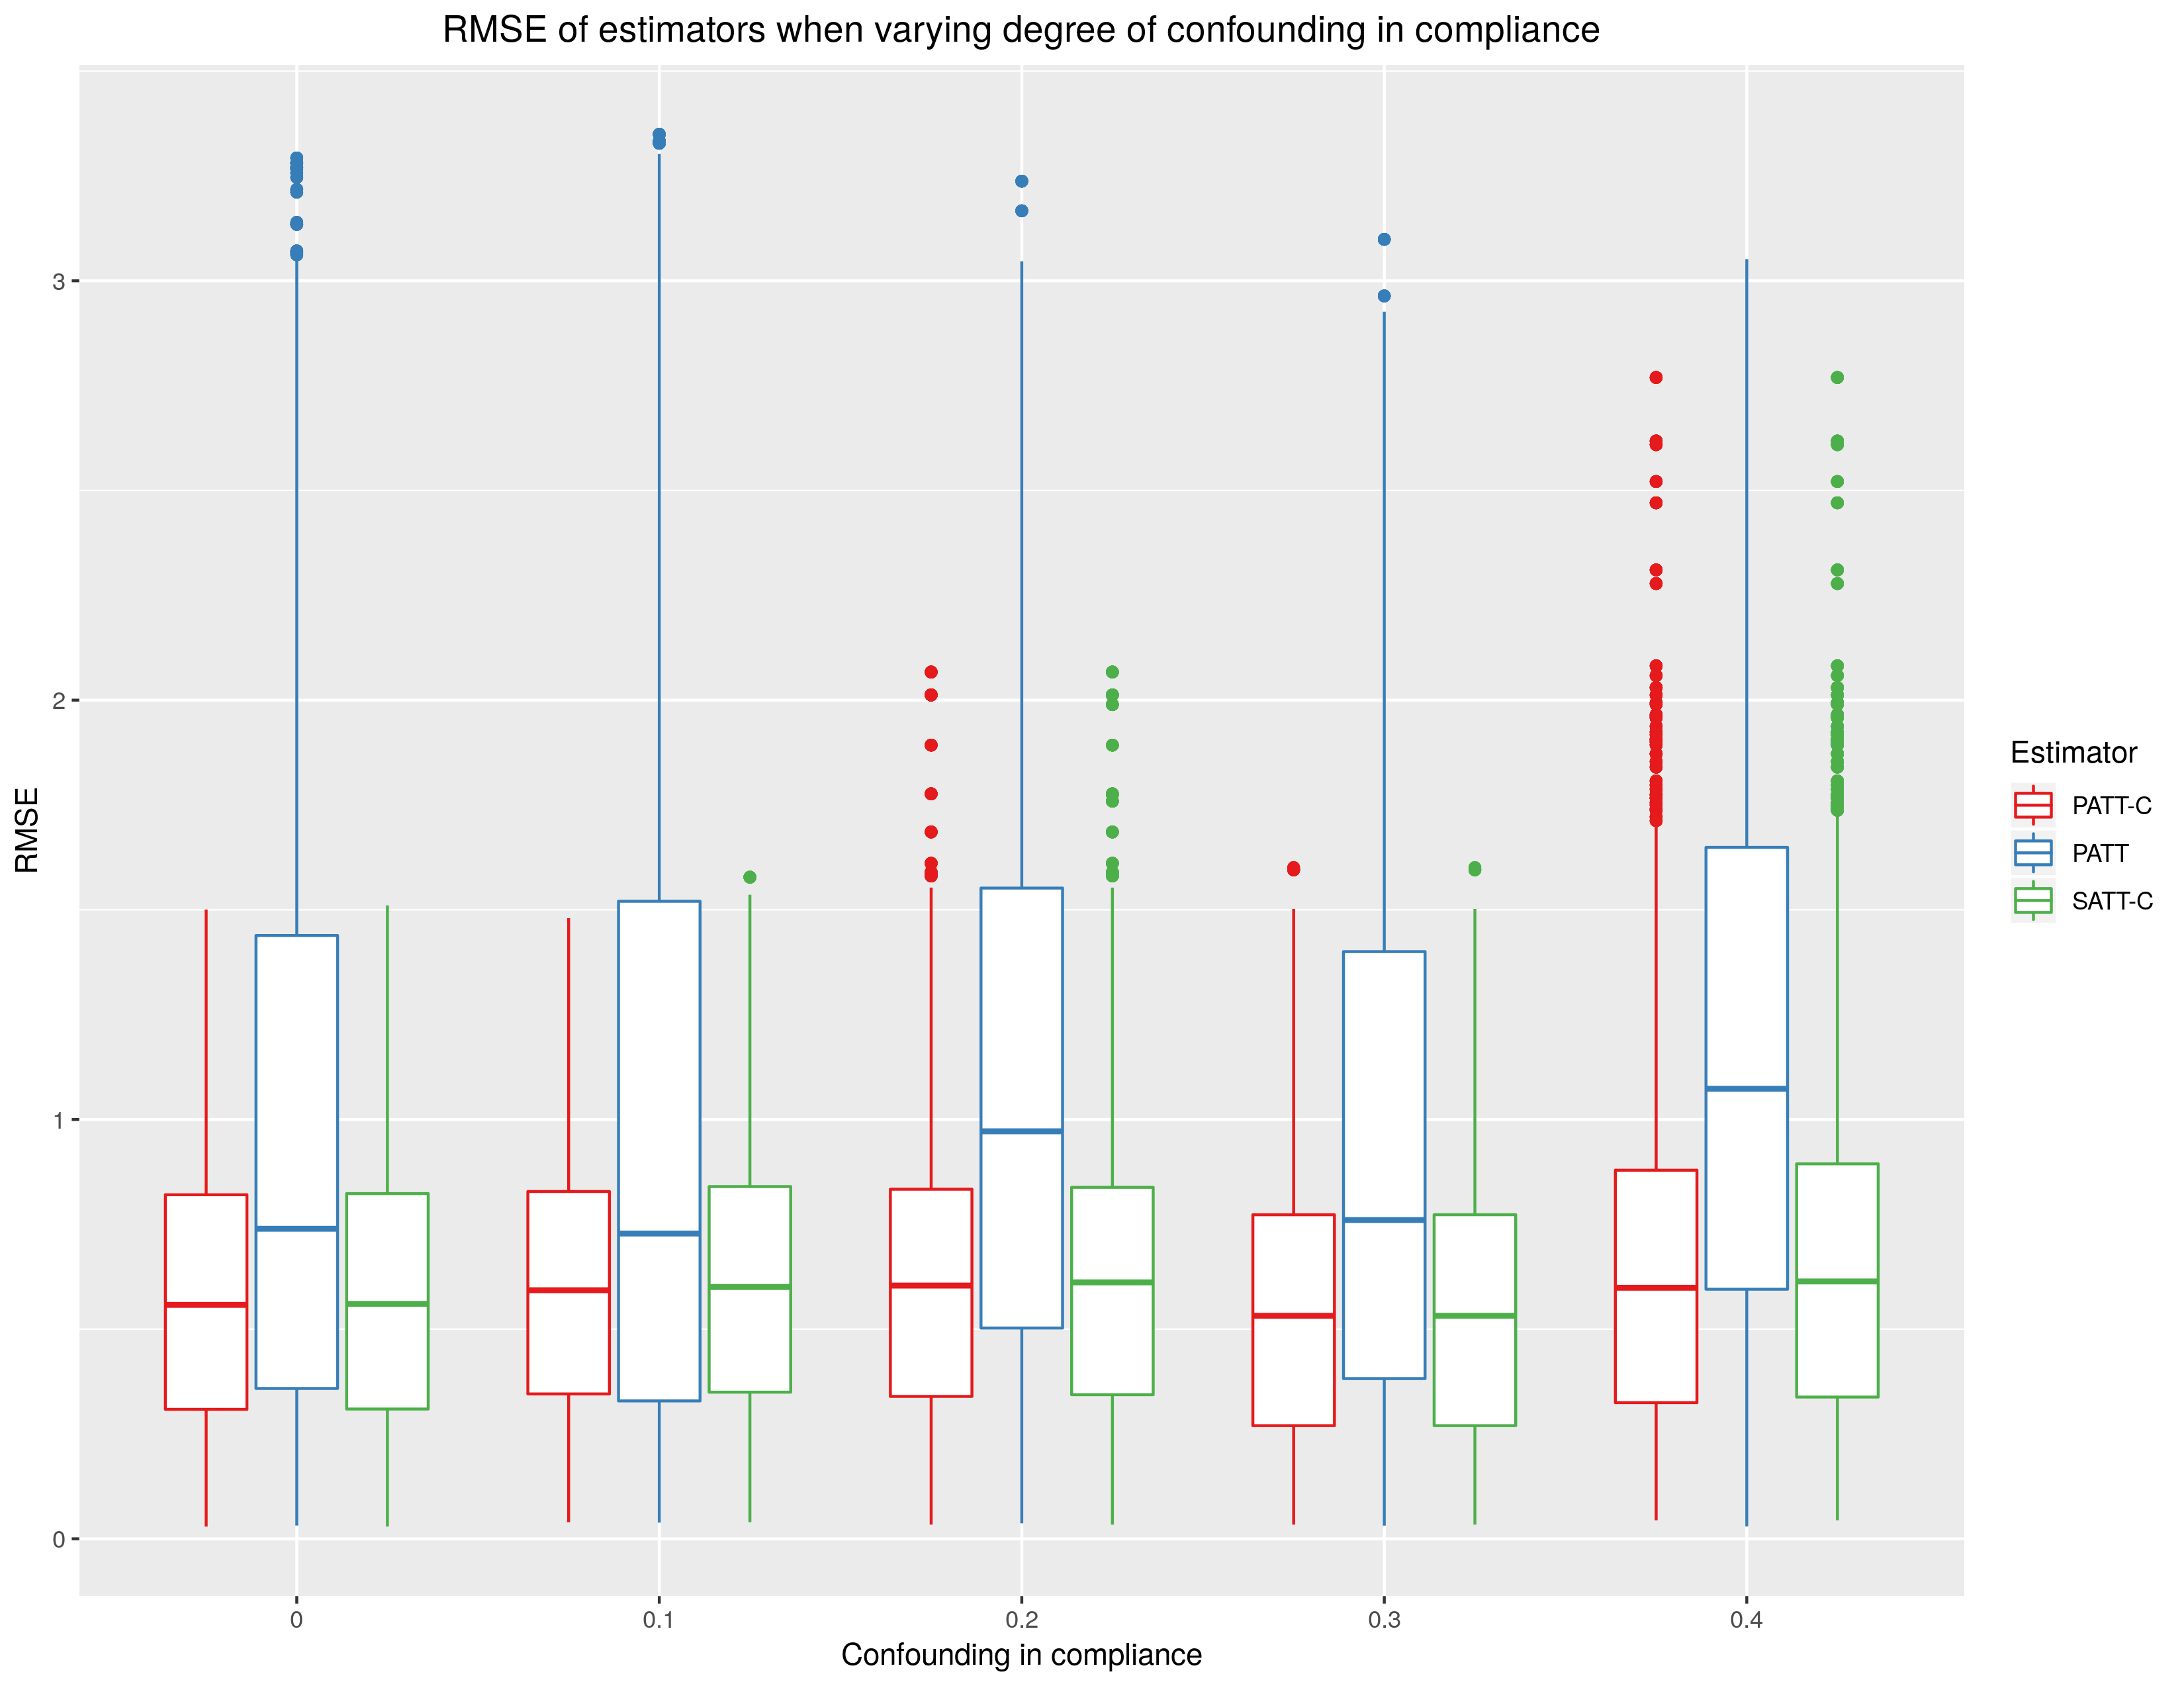
\includegraphics[width = 1\textwidth]{rmse_boxplots_RateConC.png}
		\caption{Average RMSE according to degree of confounding in compliance.\label{fig:rmse_boxplots_RateConC}}
	%	\caption{\label{fig:rmse_boxplots_RateConC} here}
	\end{center}
\end{figure}

\begin{figure}[htbp]
	\begin{center}
		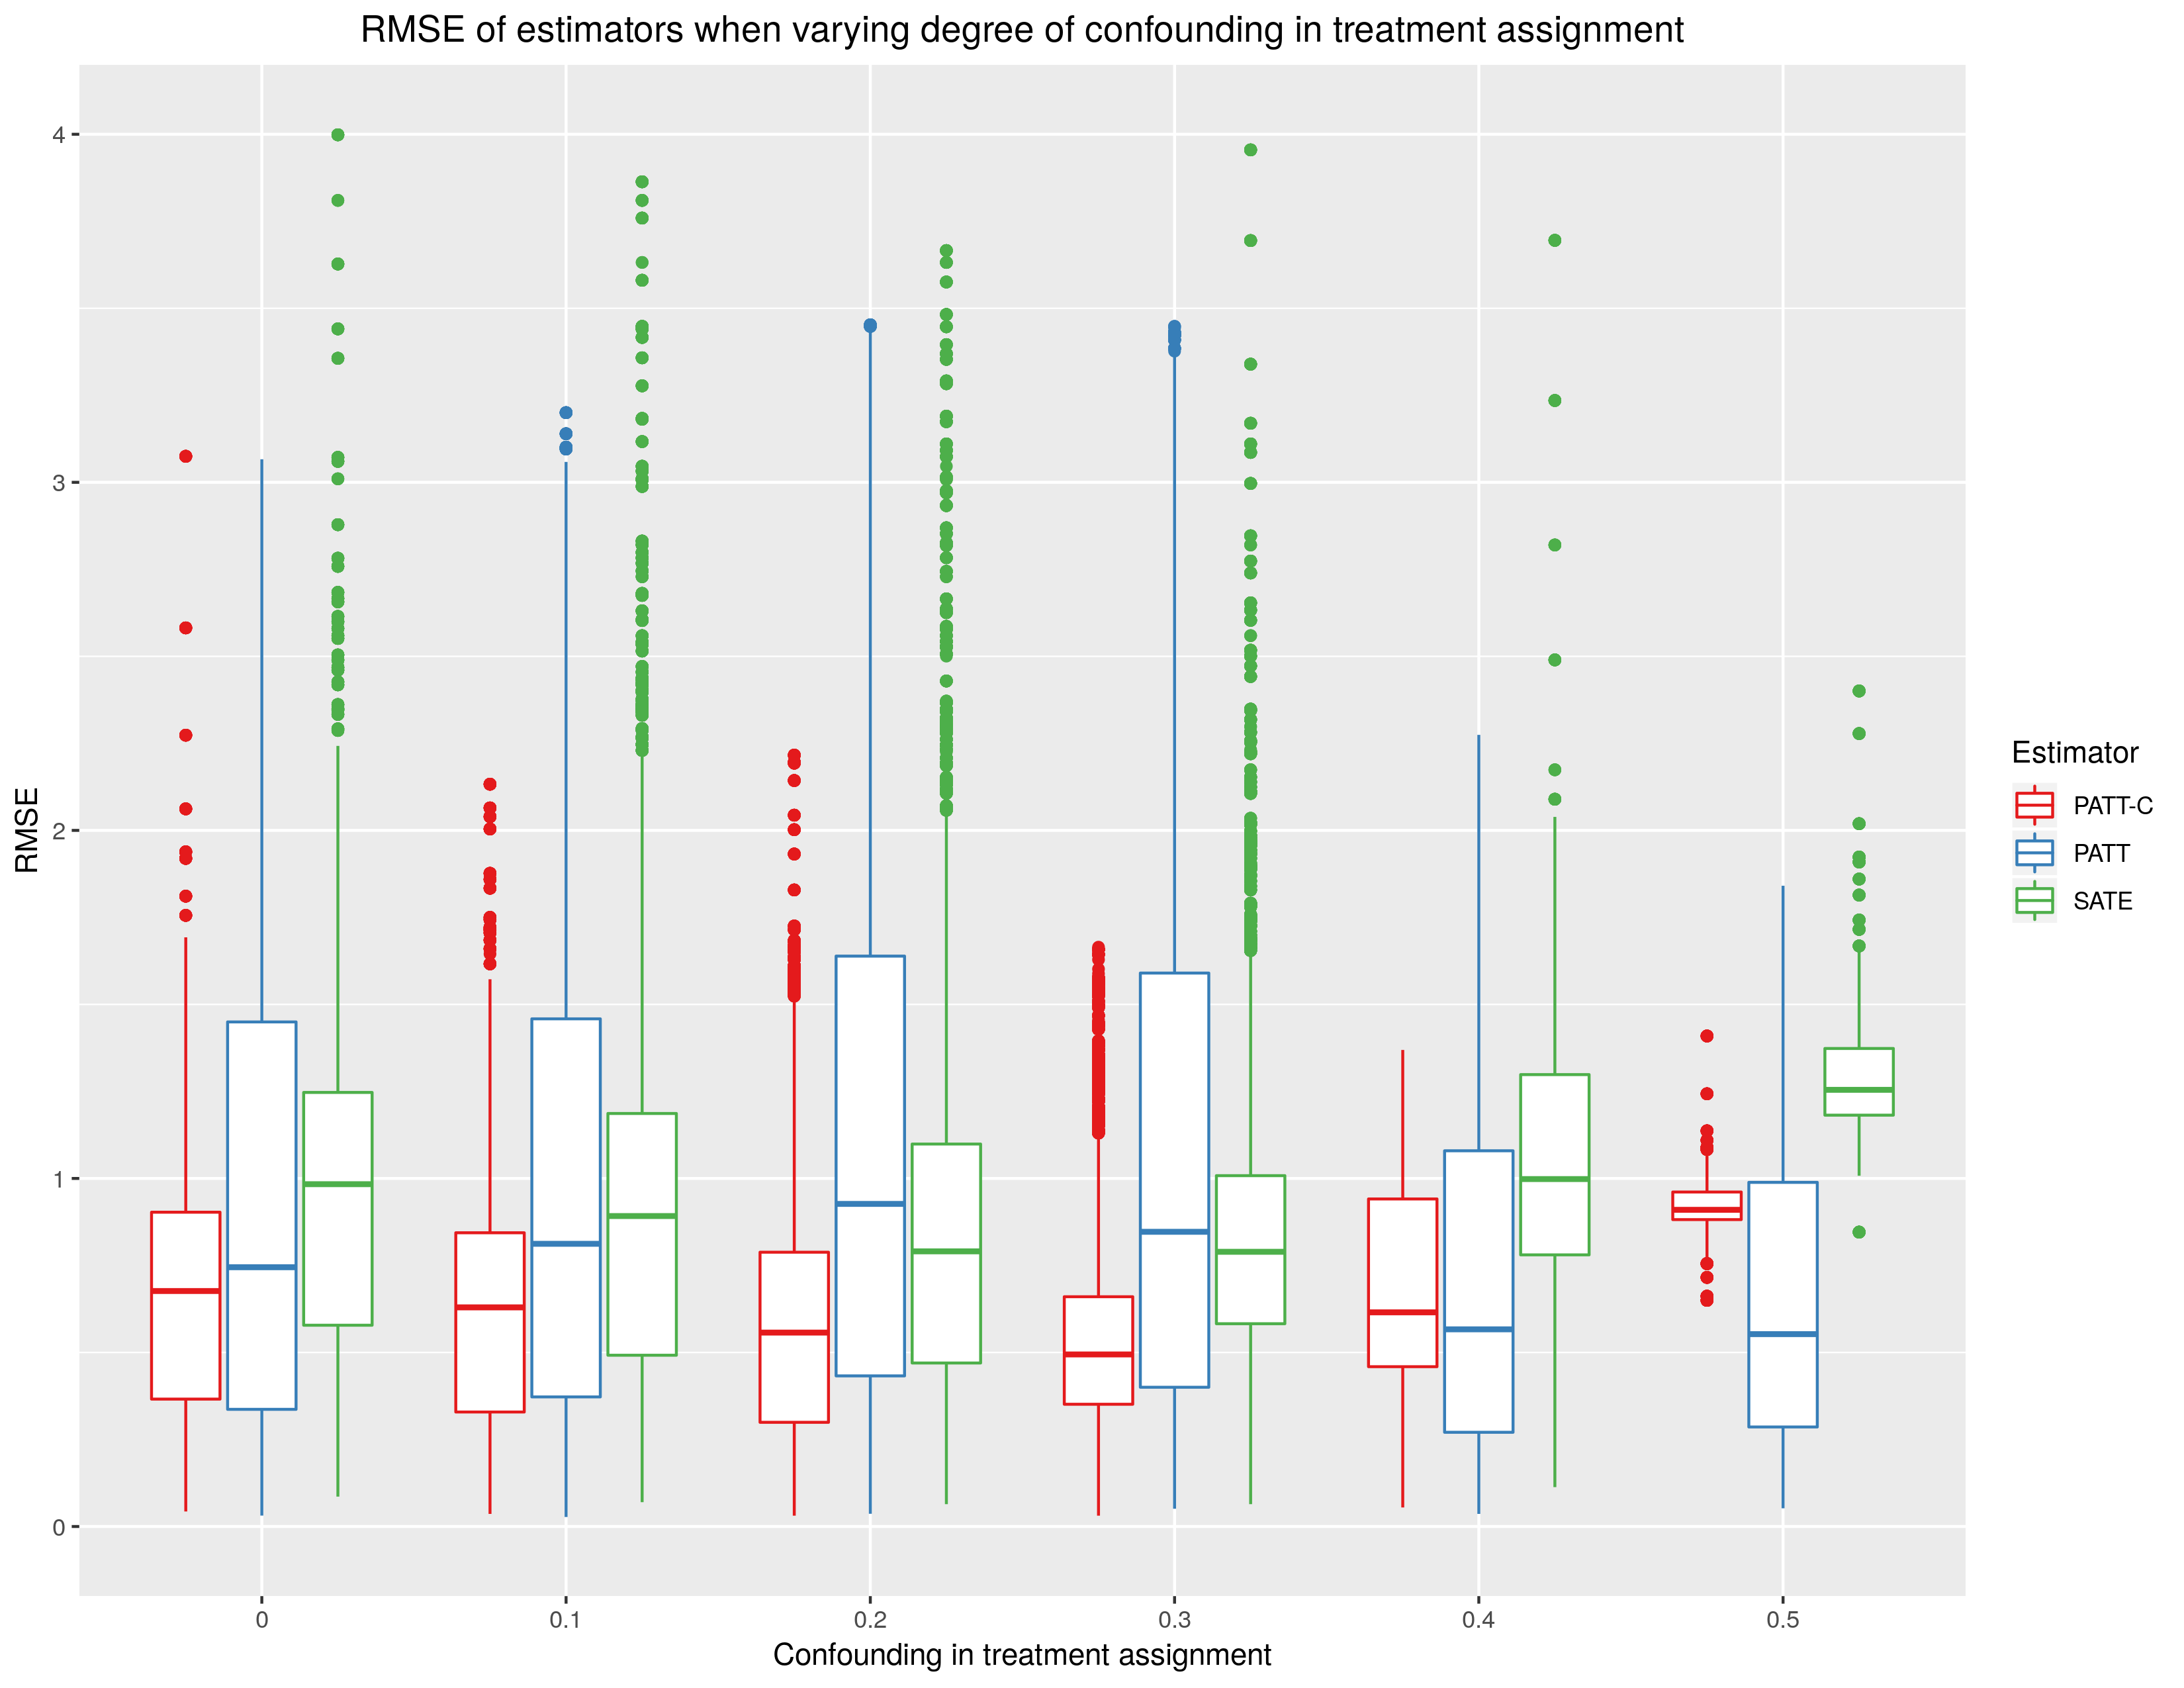
\includegraphics[width = 1\textwidth]{rmse_boxplots_RateConT.png}
		\caption{Average RMSE according to degree of confounding in treatment assignment.\label{fig:rmse_boxplots_RateConT}}
	%		\caption{\label{fig:rmse_boxplots_RateConT} here}
	\end{center}
\end{figure}

\begin{figure}[htbp]
	\begin{center}
		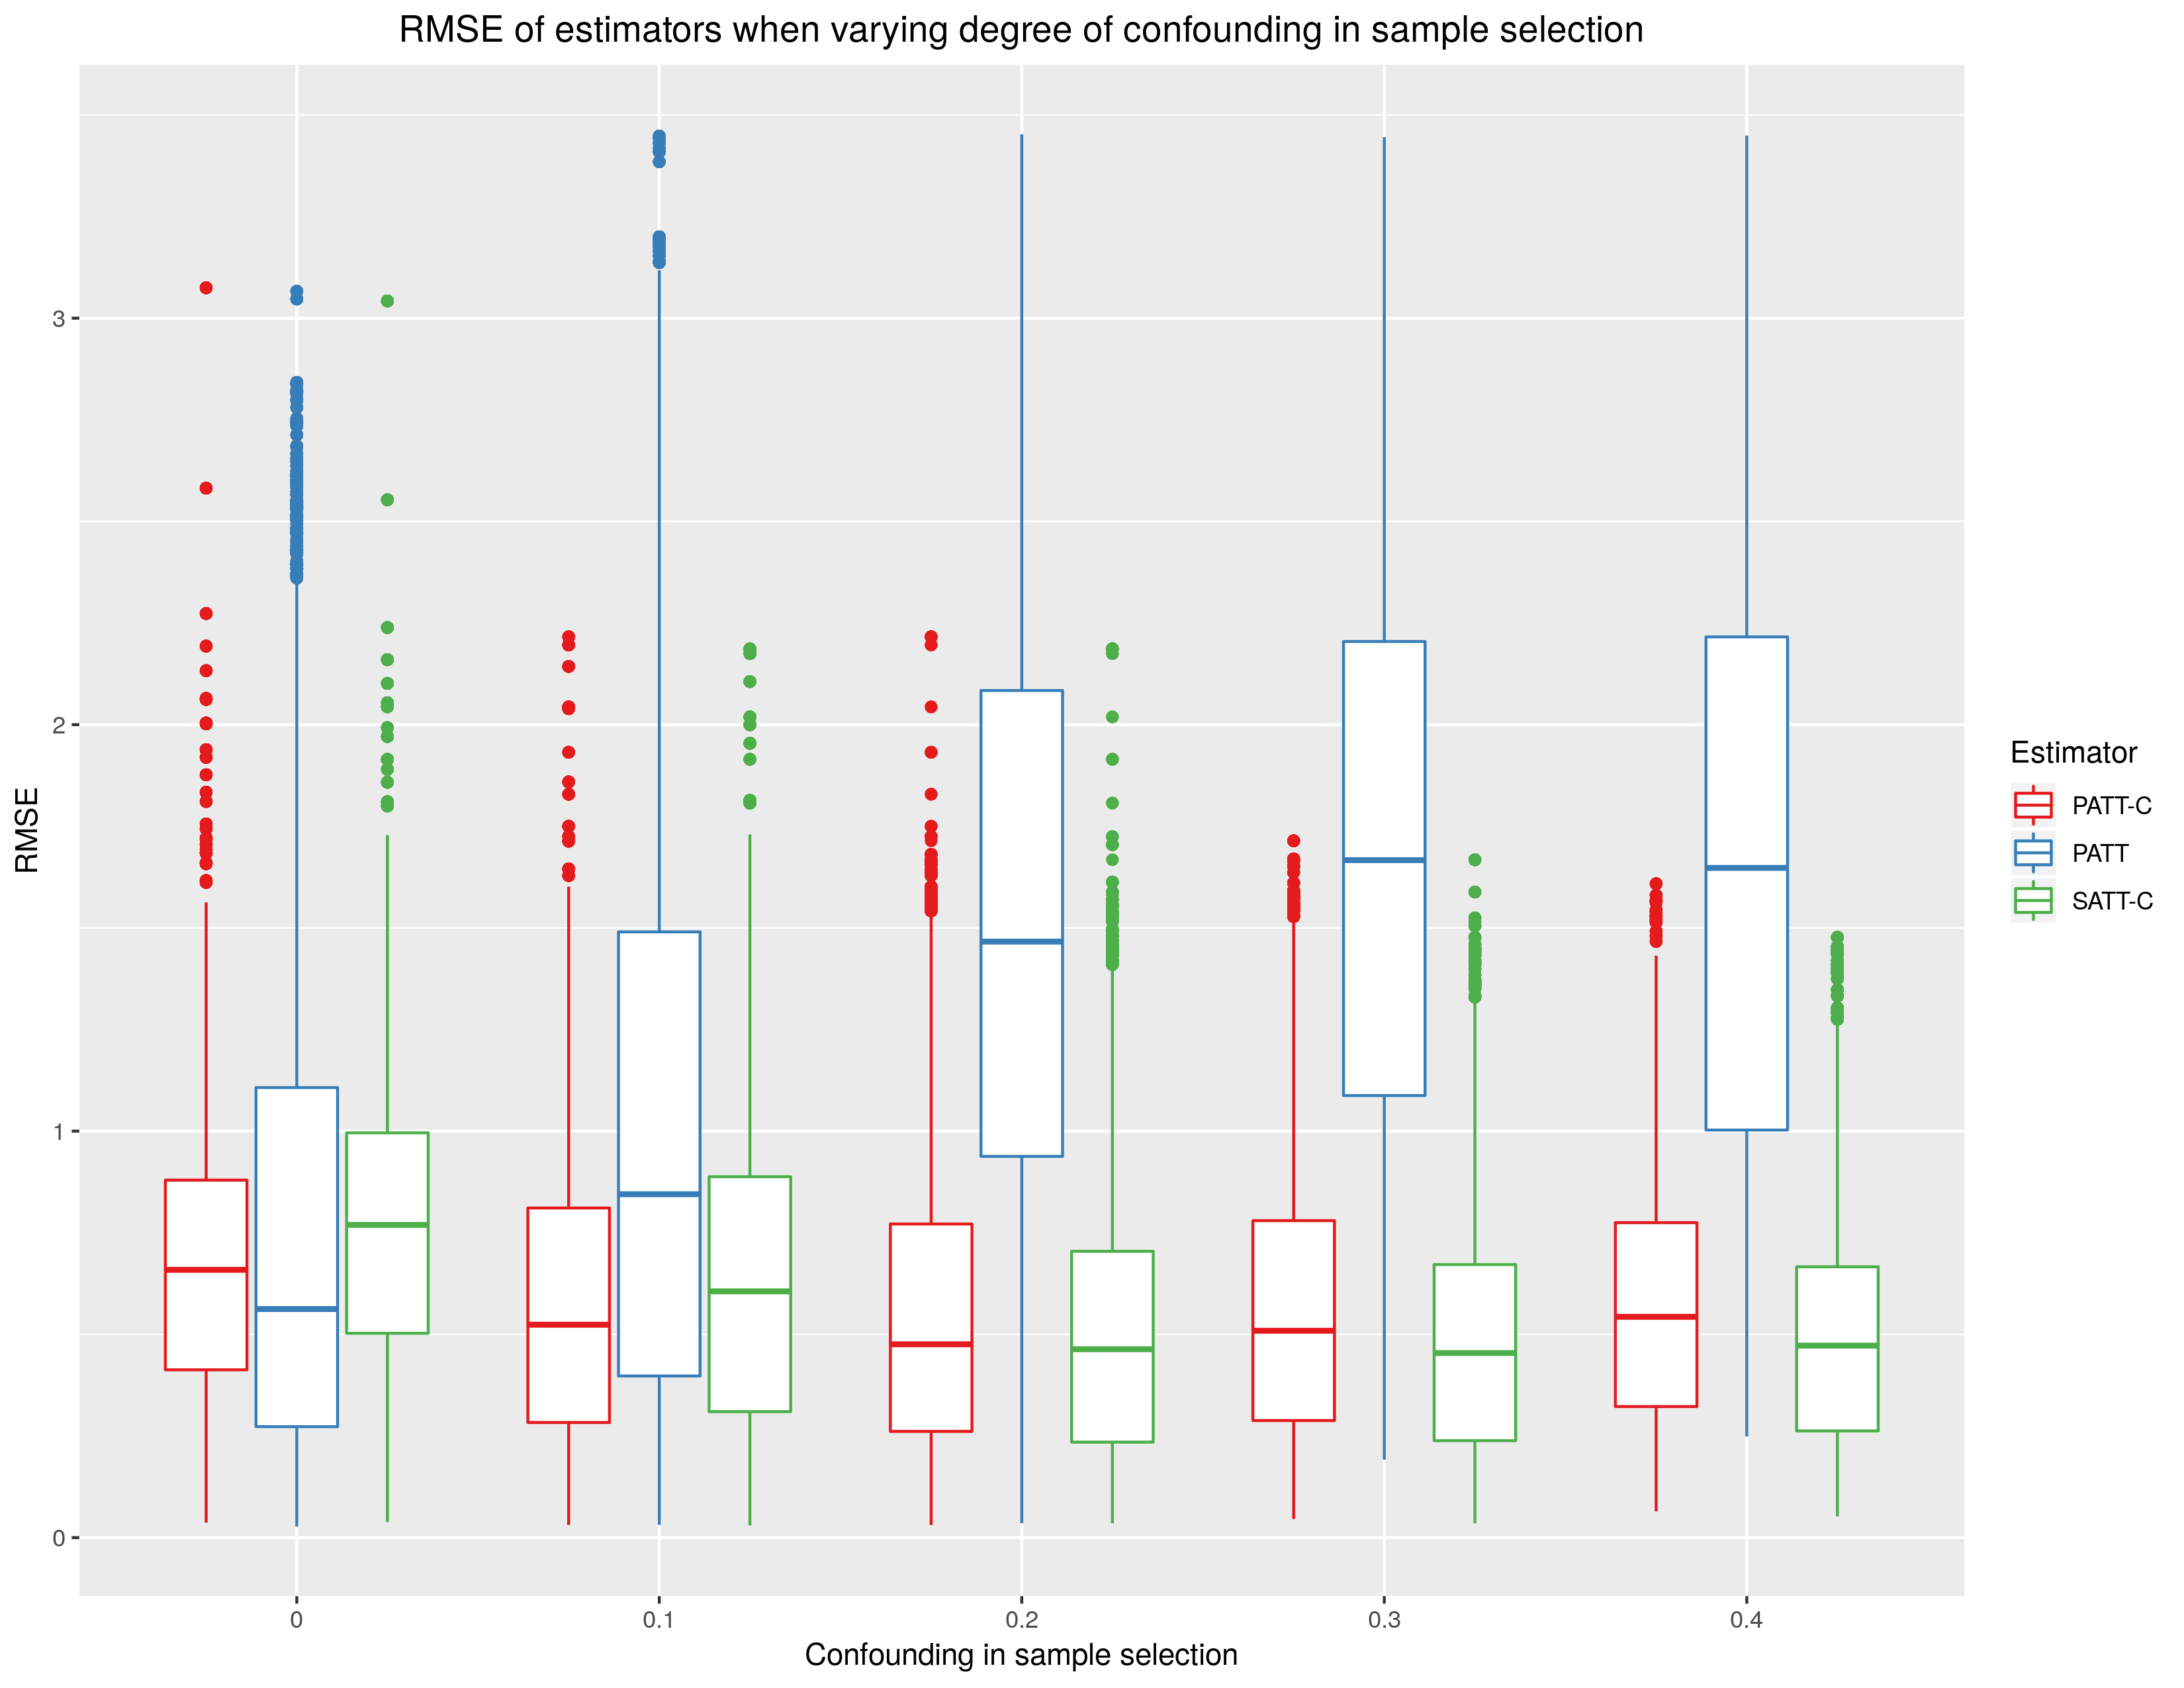
\includegraphics[width = 1\textwidth]{rmse_boxplots_RateConS.png}
		\caption{Average RMSE according to degree of confounding in sample selection.\label{fig:rmse_boxplots_RateConS}}
	%		\caption{\label{fig:rmse_boxplots_RateConS} here}
	\end{center}
\end{figure}

\newgeometry{left=3cm,bottom=0.1cm}
\begin{singlespace}
	\begin{longtable}{lllllll}
		\caption{Pretreatment covariates and responses for OHIE and NHIS respondents by Medicaid coverage status.\label{rct-nrt-compare}} \\
		& OHIE &  & OHIE &  & NHIS &  \\ 
		& no Medicaid &  & Medicaid &  &Medicaid &   \\ 
		& $n=4,519$ &  & $n=6,100$ &  & $n=6,261$ &  \\  
		\hline   
		\hline   
		\textbf{Covariate} &  N & $\mathbf{\%}$ & N & $\mathbf{\%}$ & N & $\mathbf{\%}$ \\ 
		\hline
		\textit{Sex:} &  & & &  &  & \\ 
		
		\hspace{3mm} Female & 2,538 & 56.2 & 3506 & 57.5 & 4,288 & 68.5 \\ 
		&  & & &  &  & \\ 
		\textit{Age:} &  & & &  &  & \\ 
		\hspace{3mm}19-49 & 1,288 & 28.5 & 1,625 & 26.6 & 4324 & 69.1  \\ 
		
		\hspace{3mm}50-64 & 3,231 & 71.5 & 4,475 & 73.4 & 1,937 & 30.9 \\ 
		&  & & &  &  & \\ 
		\textit{Race:} &  & & &  &  & \\ 
		\hspace{3mm}White & 3,956 & 87.5 & 5,183 & 85.0 & 3,902 & 62.3  \\ 
		
		\hspace{3mm}Black & 193 & 4.3 & 247 & 4.0 & 1,723 & 27.5  \\ 
		
		\hspace{3mm}Hispanic &  264 & 5.8 & 538 & 8.8 & 1,570 & 25.1  \\ 
		&  & & &  &  & \\ 
		\textit{Health status:} &  & & &  &  & \\ 
		\hspace{3mm}Diabetes & 459 & 10.2 & 637 & 10.4 & 866 & 13.8  \\ 
		
		\hspace{3mm}Asthma & 823 & 18.2 & 1,094 & 17.9 & 1272 & 20.3   \\ 
		
		\hspace{3mm}High blood pressure & 1,362 & 30.1 & 1,705 & 27.9 & 2,166 & 34.6  \\ 
		
		\hspace{3mm}Heart condition & 120 & 2.7 & 189 & 3.1 & 529 & 8.4 \\ 
		&  & & &  &  & \\ 
		\textit{Education:} &  & & &  &  & \\  
		\hspace{3mm}Less than high school  & 858 & 19.0 & 1,154 & 18.9 & 1,942 & 31.0  \\ 
		
		\hspace{3mm}High school diploma or GED & 2,589 & 57.3 & 3,279 & 53.8 & 2,076 & 33.2   \\ 
		
		\hspace{3mm}Voc. training / 2-year degree & 804 & 17.8 & 1,186 & 19.4 & 1,810 & 28.9  \\ 
		
		\hspace{3mm}4-year college degree or more & 268 & 5.9 & 481 & 7.9 & 433 & 6.9  \\ 
		&  & & &  &  & \\ 
		\textit{Income:} &  & & &  &  & \\ 
		\hspace{3mm} $<\$10$k & 4,518 & 100.0 & 4,111 & 67.4 & 2,588 & 41.3  \\
		
		\hspace{3mm} \$10k-\$25k & 1 & 0.0 & 1,616 & 26.5 & 3,098 & 49.5 \\
		
		\hspace{3mm} $>\$25$k & 0 & 0.0 & 373 & 6.1 & 575 & 9.2   \\
		\hline
		\hline
%		\textbf{Binary response} &  $\mathbf{n}$ & $\mathbf{\%}$ & $\mathbf{n}$ & $\mathbf{\%}$ & $\mathbf{n}$ & $\mathbf{\%}$ \\ 
%		\hspace{3mm}Any ER visit &  1,377 & 25.4 & 1,301 & 25.1 & 1,659 & 26.5  \\  
%		%\hspace{3mm}Any outpatient visit & 3,265 & 60.2 & 3,081 & 59.3 & 4,093 & 65.4 \\
%		\hline
		\textbf{Responses} &  Mean & S.d. & Mean & S.d. & Mean & S.d. \\  
		\hspace{3mm}$\#$ ER visits &  0.44 & 0.95 & 0.44 & 0.99 & 0.48 & 1.0  \\  
		\hspace{3mm}$\#$ outpatient visits & 1.9 & 3.01 & 1.9 & 2.8 & 2.08 & 2.3 \\
		\hline
		\hline
	\end{longtable}
\noindent
\footnotesize{Notes: weighted using OHIE (first two columns) or NHIS (last column )survey weights.}
\end{singlespace}
\restoregeometry

\begin{table}[h]
	\caption{Distribution of OHIE participants by status of treatment assignment ($T_i$) and treatment received ($D_i$).\label{ohie-status}} 
	\begin{tabular}{@{}lccc@{}}
		\toprule
		& $D_i = 0$ & $D_i = 1$ & n      \\ \midrule
		$T_i = 0$ & 10,010    & 1,556     & 11,566 \\
		$T_i = 1$ & 6,446     & 5,193     & 11,639 \\
		n         & 16,456    & 6,749     & 23,205 \\ \bottomrule
	\end{tabular}\\ \\
	\footnotesize{Notes: weighted using OHIE survey weights.}
\end{table}

\begin{table}[h]
		\caption{Placebo test results comparing the mean outcomes of RCT compliers and adjusted \textcolor{red}{population members who received treatment}.\label{placebo}} 
	\begin{tabular}{@{}lcccc@{}}
		\toprule
		Outcome                & RCT complier & Adjusted population & Difference & Per-comparison \\
				               &  mean 		  & mean 					  & 		   & $p$-value \\		
		 \midrule
	%	Any ER visit           & 0.25              & 0.25                           & 0.0001     & 0.97  \\
		$\#$ ER vists          & 0.45              & 0.45                           & 0.002      & 0.85   \\
		$\#$ outpatient visits & 1.90              & 1.94                           & -0.03      & 0.26   \\ \bottomrule
	\end{tabular}\\ \\
\footnotesize{Notes: survey-weighted difference-in-means $p$-values calculated from two-sided t-test.}
\end{table}

\begin{table}[h]
	\caption{Comparison of population and sample estimates.\label{compliance-compare}} 
	\begin{tabular}{@{}llll@{}}
		\toprule
		\backslashbox{Estimator}{Outcome} 				& Any ER visit 	& $\#$ ER visits   & $\#$ outpatient visits      \\ \midrule
		PATT-C                                           & 0.0001 [0.0001, 0.0001]   & 0.0005 [0.0002, 0.0008]	& 0.002 [0.002, 0.002] \\
		PATT                                             & 0.0006 [0.0005, 0.0007]   & -0.004 [-0.005, -0.004]	& 0.02 [0.02, 0.02]  \\
		CACE                                             & -0.001 [-0.02, 0.02]   & 0.005 [-0.05, 0.06]	& -0.02 [-0.19, 0.14]  \\ \bottomrule
	\end{tabular}\\
	\footnotesize{Notes: Estimates in brackets represent 95\% bootstrap confidence intervals constructed with 1,000 bootstrap samples.}
\end{table}

\begin{figure}[htbp]
	\begin{center}
		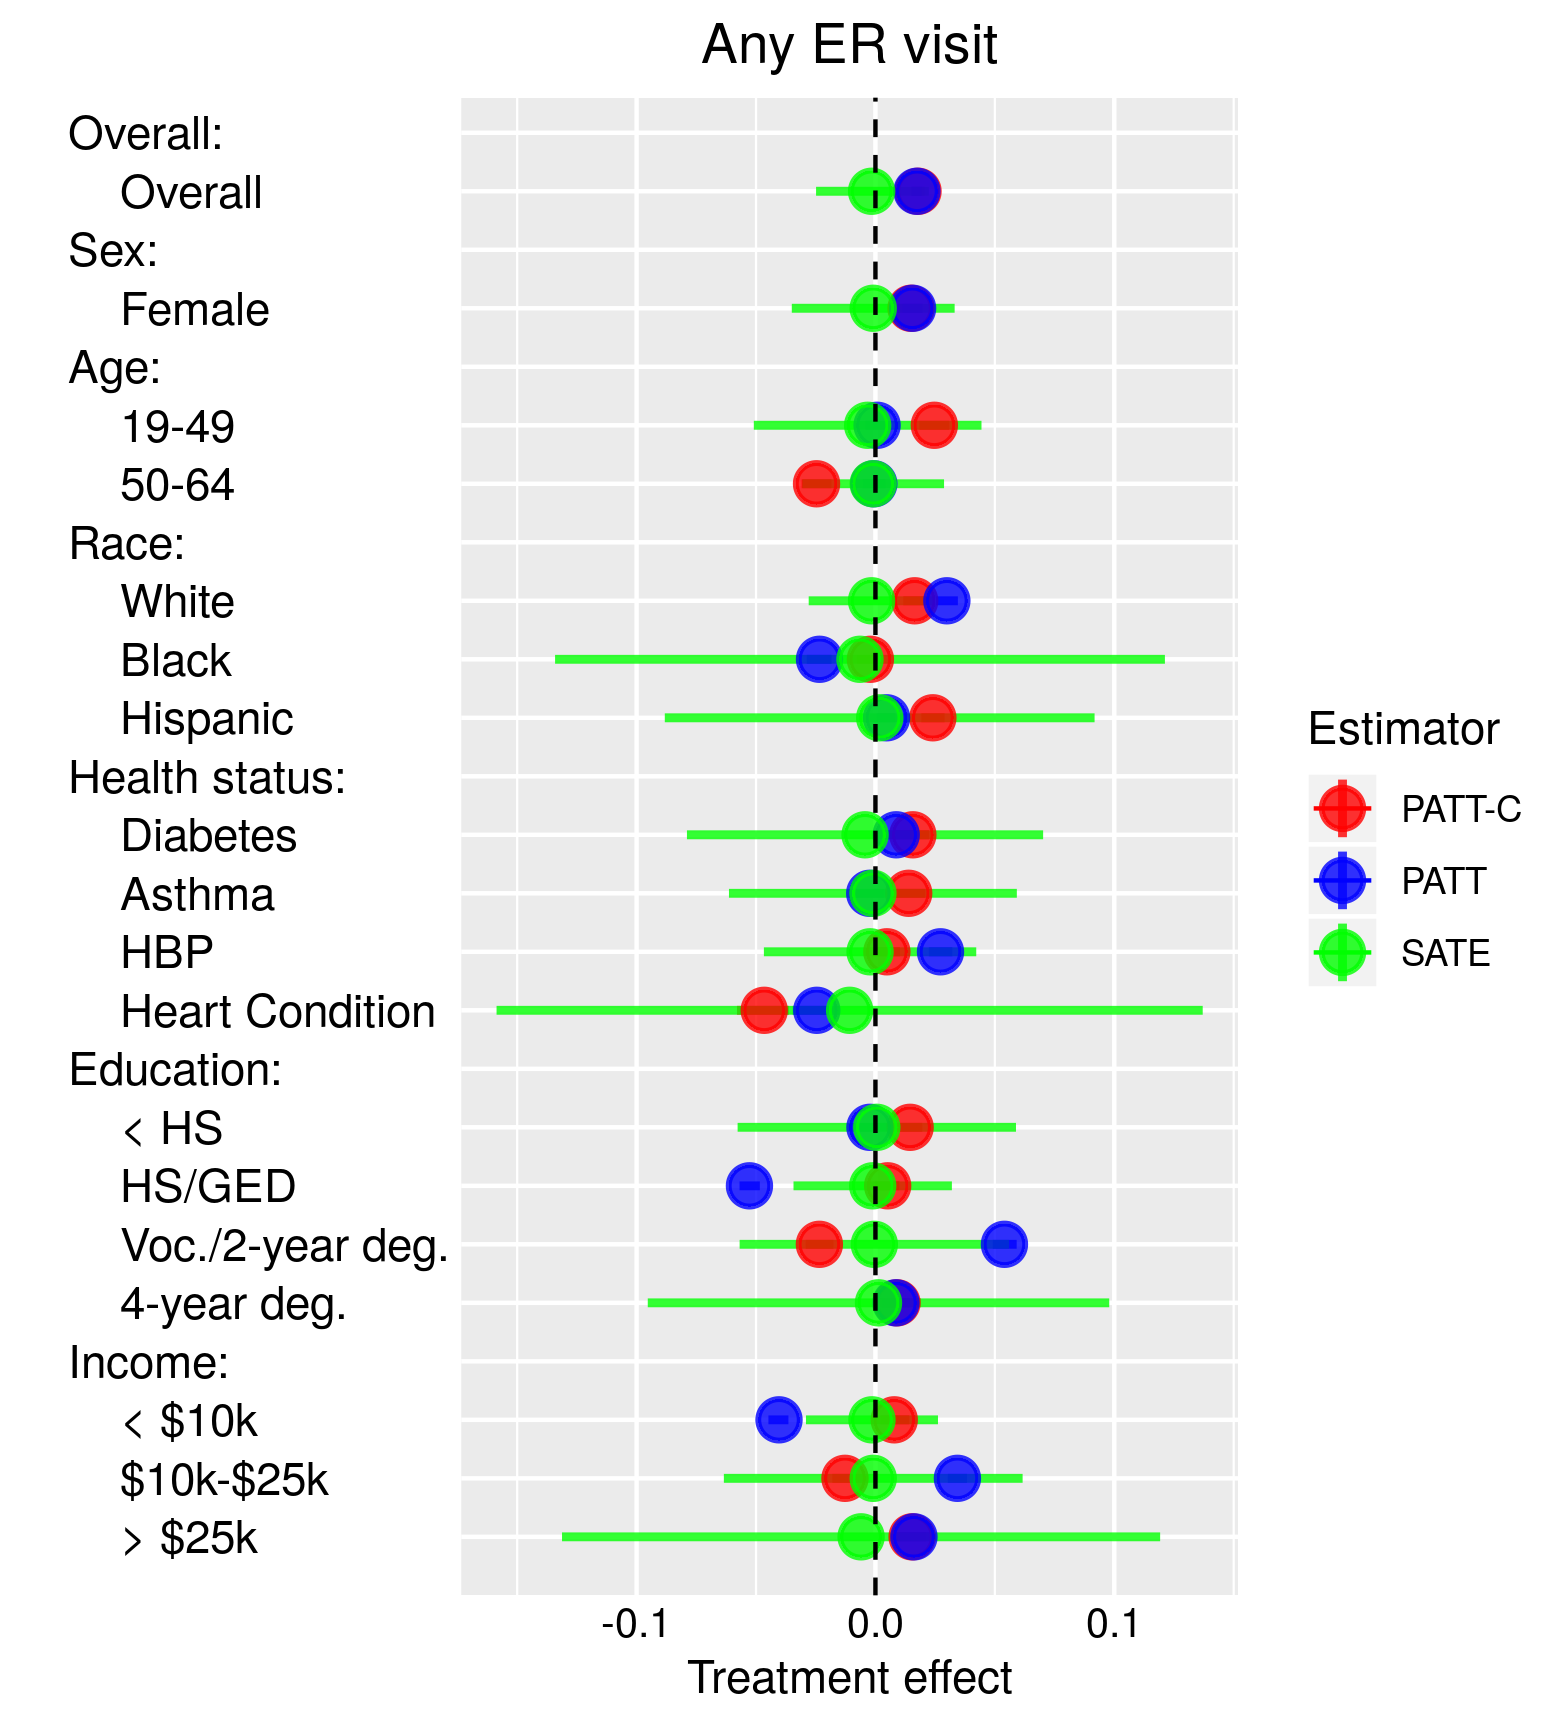
\includegraphics[width = 0.9\textwidth]{any-visit-plot.png}
		\caption{Heterogeneity in sample and population treatment effect estimates: any ER visit. Horizontal lines represent 95\% bootstrap confidence intervals constructed with 1,000 bootstrap samples.\label{fig:any-visit-plot}}
		%	\caption{\label{fig:any-visit-plot} here}
	\end{center}
\end{figure}


\begin{figure}[htbp]
	\begin{center}
		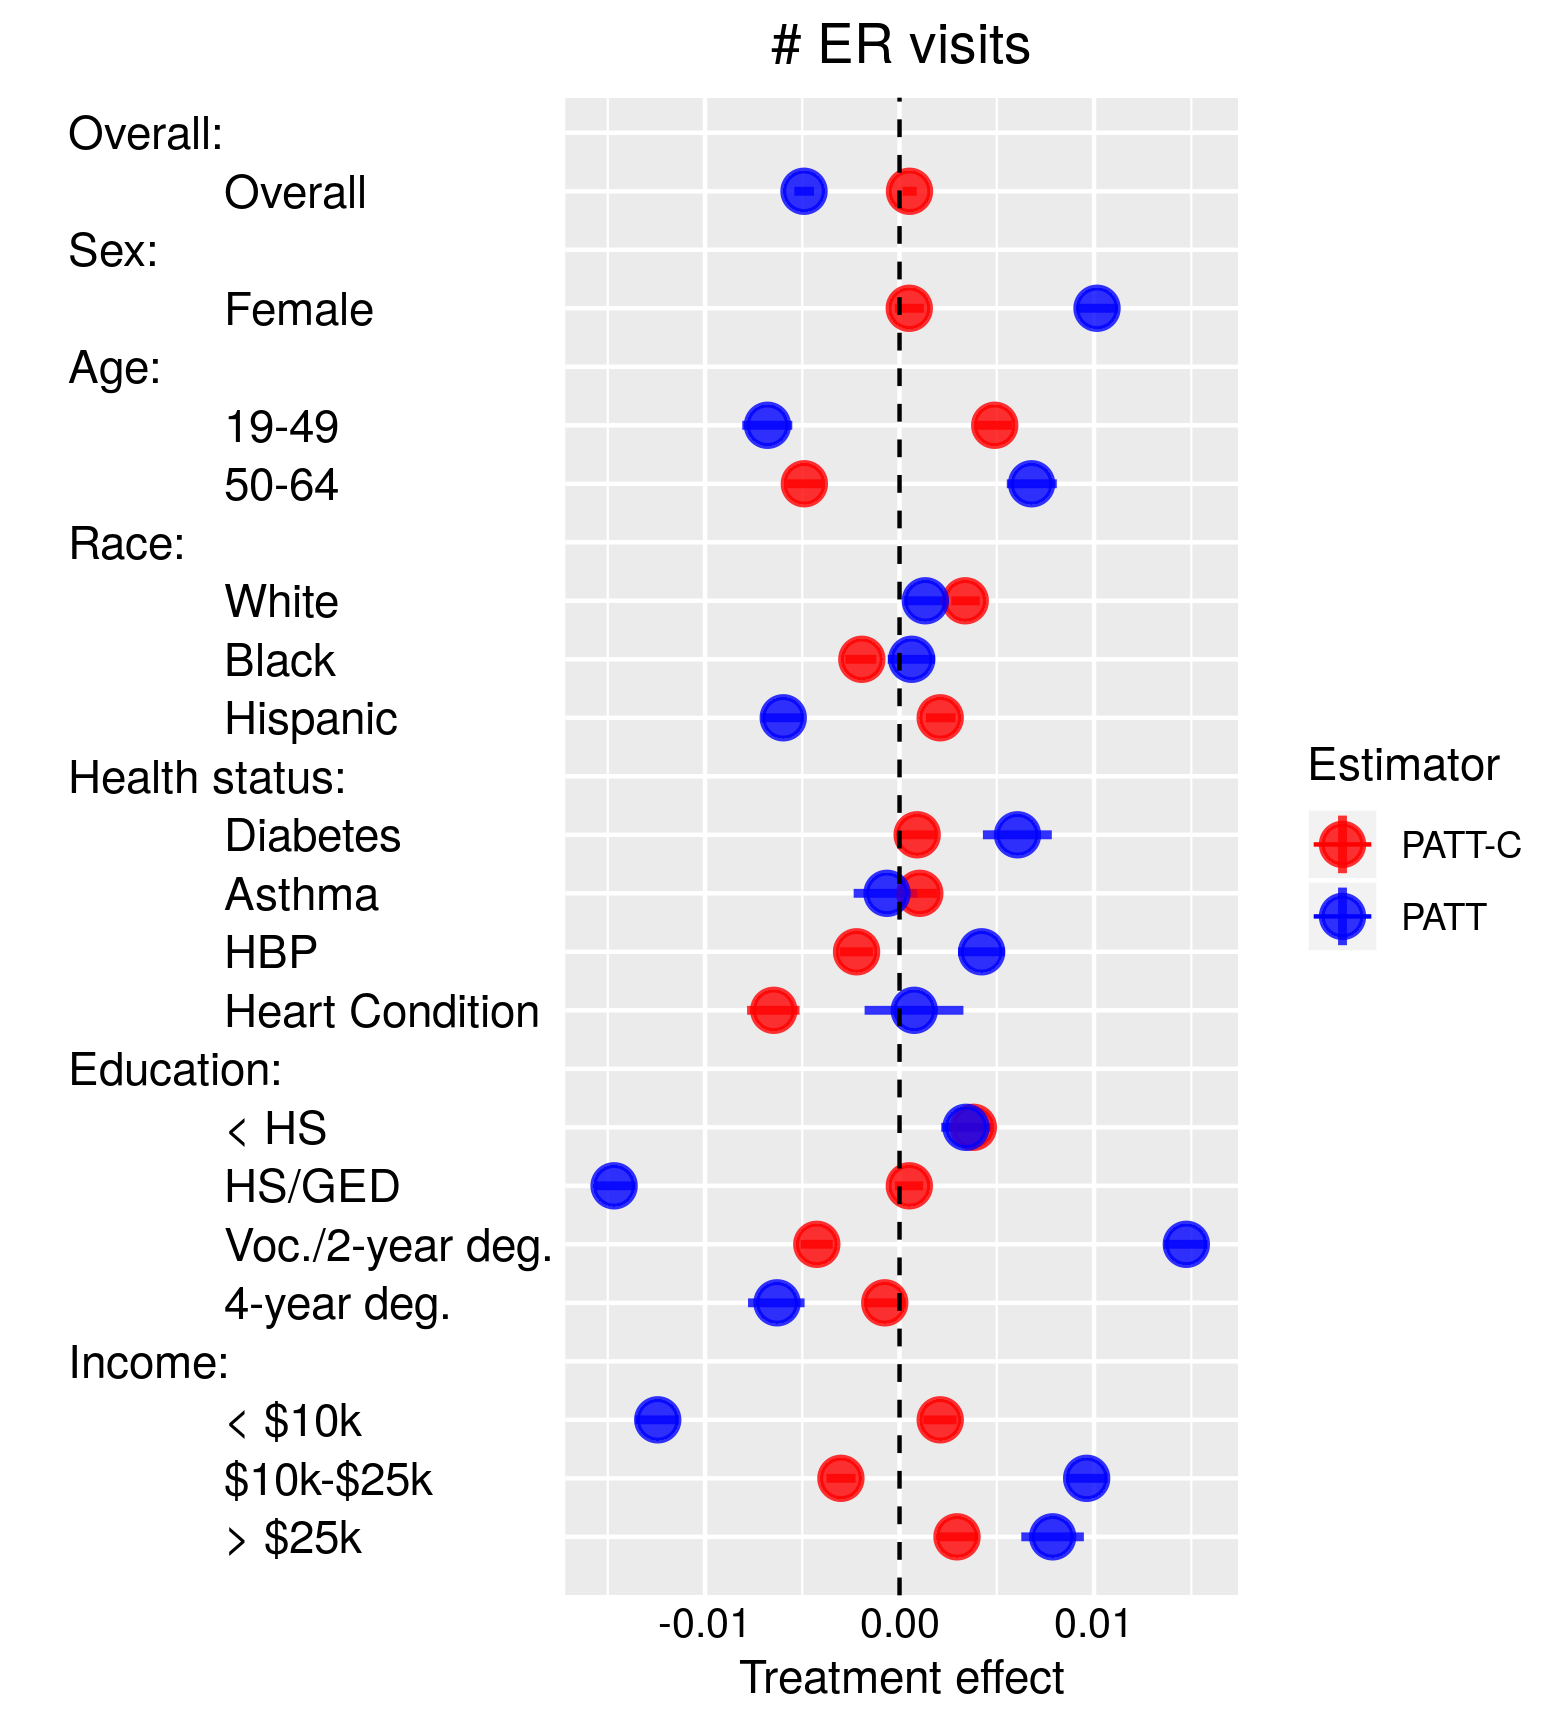
\includegraphics[width = 0.9\textwidth]{num-visit-plot.png}
		\caption{Heterogeneity in population treatment effect estimates: $\#$ ER visits.\label{fig:num-visit-plot}}
		%	\caption{\label{fig:num-visit-plot} here}
	\end{center}
\end{figure}

\begin{figure}[htbp]
	\begin{center}
		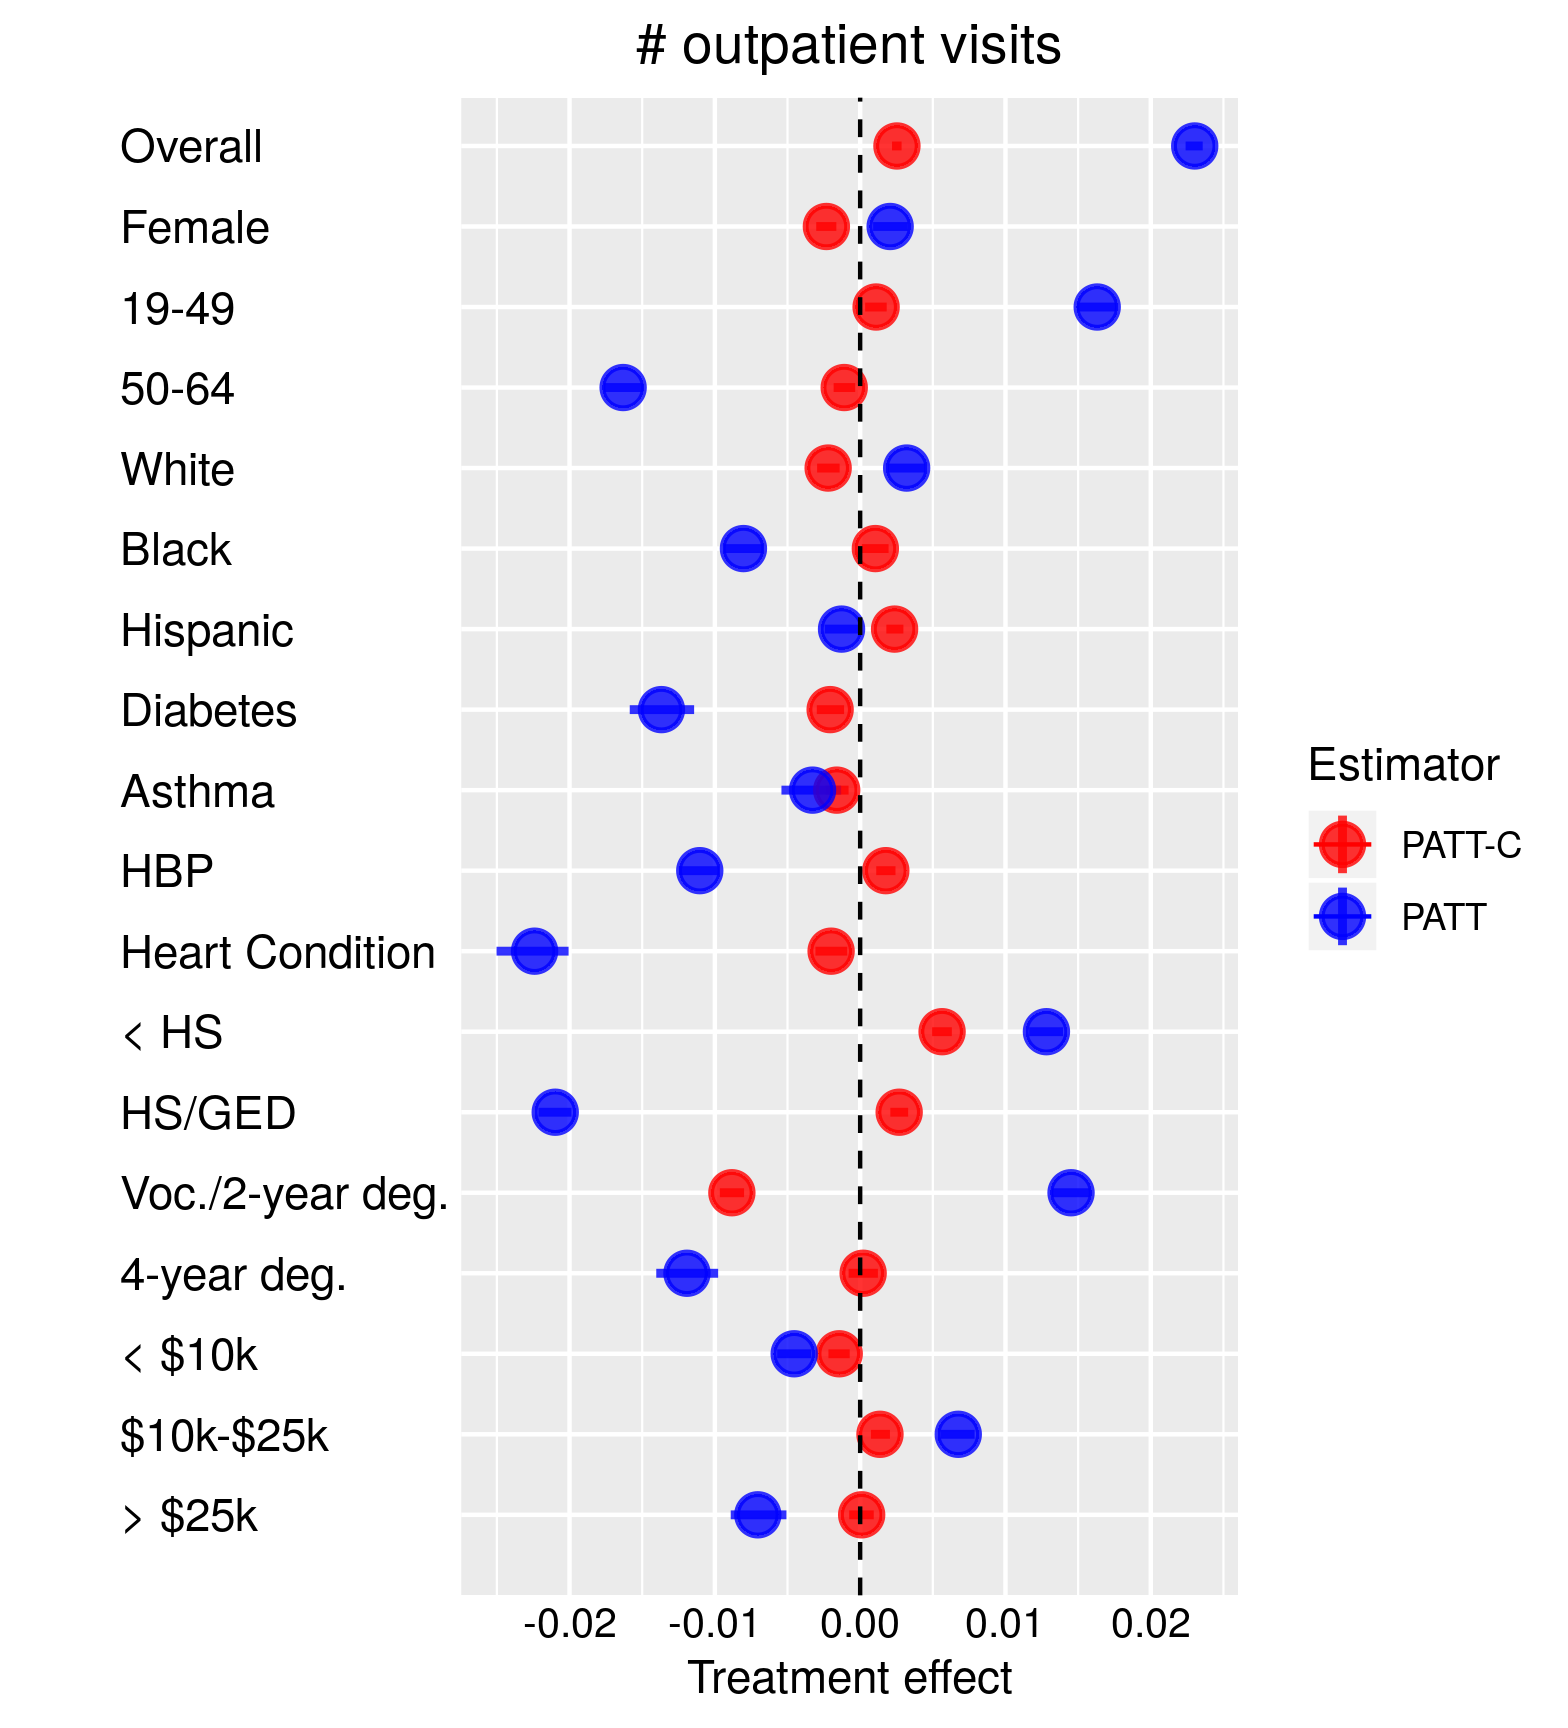
\includegraphics[width = 0.9\textwidth]{num-out-plot.png}
		\caption{Heterogeneity in population treatment effect estimates: $\#$ outpatient visits.\label{fig:num-out-plot}}
		%	\caption{\label{fig:num-out-plot} here}
	\end{center}
\end{figure}

% complier-mod
\begin{table}[h]
\begin{center}
\caption{Distribution of MSE for compliance ensemble.\label{compliance-ensemble}} 
\begin{tabular}{lcccc}
  \hline
 Algorithm & Mean & SE & Min. & Max. \\ 
  \hline
        \rowcolor{Gray}
Super learner (\texttt{SuperLearner}) & 0.22  & 0.001 & 0.21 & 0.23 \\
%Discrete SL & 0.22  & 0.001 & 0.21 & 0.23 \\
Lasso regression (\texttt{glmnet})  & 0.22  & 0.001 & 0.21 & 0.23 \\
Random forests (\texttt{randomForest}) & 0.27  & 0.002 & 0.25 & 0.29 \\
Ridge regression (\texttt{glmnet}) & 0.22  & 0.001 & 0.21 & 0.23 \\
   \hline
\end{tabular} 
\end{center}
\footnotesize{Notes: MSE is 10-fold cross-validated error for super learner ensemble and candidate algorithms. \textsf{R} package used for implementing each algorithm in parentheses.}
\end{table}

\pagebreak

\begin{table}[h]
\caption{Error and weights for candidate algorithms in response ensemble for RCT compliers.\label{reponse-ensemble}}  
  \begin{tabularx}{\linewidth}{l*{3}{Y}}
    \toprule
    \multicolumn{3}{l}{\textbf{Any ER visit}} \\
    \midrule
 Algorithm &  MSE & Weight \\ 
  \hline
Lasso regression (\texttt{glmnet})  & 0.18 & 1 \\ 
Random forests, $\# preds. = 1$ (\texttt{randomForest}) & 0.25 & 0 \\ 
Random forests, $\# preds. = 10$ (\texttt{randomForest}) & 0.24 & 0 \\ 
Regularized logistic regression, $\alpha=0.25$ (\texttt{glmnet})  & 0.19 & 0 \\ 
Regularized logistic regression, $\alpha=0.5$ (\texttt{glmnet})  & 0.19 & 0 \\ 
Regularized logistic regression, $\alpha=0.75$ (\texttt{glmnet})  & 0.19 & 0 \\ 
Ridge regression (\texttt{glmnet})  & 0.18 & 0 \\ 
   \hline
  \end{tabularx}
  \begin{tabularx}{\linewidth}{l*{3}{Y}}
    \toprule
    \multicolumn{3}{l}{\textbf{$\#$ ER visits}} \\
    \midrule
Algorithm  & MSE & Weight \\ 
\hline
Additive regression, $\text{degree} = 3$ (\texttt{gam})  & 0.95 & 0 \\ 
Additive regression, $\text{degree} = 4$ (\texttt{gam})  & 0.95 & 0 \\ 
Lasso regression (\texttt{glmnet})  & 0.95 & 0.92 \\ 
Random forests, $\# preds. = 1$ (\texttt{randomForest}) & 0.95 & 0 \\ 
Random forests, $\# preds. = 10$ (\texttt{randomForest}) & 0.99 & 0.08 \\ 
Regularized linear regression, $\alpha=0.25$ (\texttt{glmnet})  & 0.95 & 0 \\ 
Regularized linear regression, $\alpha=0.5$ (\texttt{glmnet})  & 0.95 & 0 \\ 
Regularized linear regression, $\alpha=0.75$ (\texttt{glmnet})  & 0.95 & 0 \\ 
Ridge regression (\texttt{glmnet})  & 0.18 & 0 \\ 
   \hline
    \bottomrule
  \end{tabularx}
  \begin{tabularx}{\linewidth}{l*{3}{Y}}
	\toprule
	\multicolumn{3}{l}{\textbf{$\#$ outpatient visits}} \\
	\midrule
	Algorithm  & MSE & Weight \\ 
	\hline
	Additive regression, $\text{degree} = 3$ (\texttt{gam})  & 8.40 & 0 \\ 
	Additive regression, $\text{degree} = 4$ (\texttt{gam})  & 8.40 & 0 \\ 
	Lasso regression (\texttt{glmnet})  & 8.38 & 0 \\ 
	Random forests, $\# preds. = 1$ (\texttt{randomForest}) & 8.38 & 0 \\ 
	Random forests, $\# preds. = 10$ (\texttt{randomForest}) & 8.79 & 0.08 \\ 
	Regularized linear regression, $\alpha=0.25$ (\texttt{glmnet})  & 8.38 & 0 \\ 
	Regularized linear regression, $\alpha=0.5$ (\texttt{glmnet})  & 8.38 & 0 \\ 
	Regularized linear regression, $\alpha=0.75$ (\texttt{glmnet})  & 8.38 & 0.92 \\ 
	Ridge regression (\texttt{glmnet})  & 8.38 & 0 \\ 
	\hline
	\bottomrule
\end{tabularx}
\footnotesize{Notes: cross-validated error and weights used for each algorithm in super learner ensemble. \textit{MSE} is the ten-fold cross-validated mean squared error for each algorithm. \textit{Weight} is the coefficient for the Super Learner, which is estimated using non-negative least squares based on the Lawson-Hanson algorithm. \textsf{R} package used for implementing each algorithm in parentheses. $\# preds.$ is the number of predictors randomly sampled as candidates in each decision tree in random forests algorithm. $\alpha$ is a parameter that mixes L1 and L2 norms. $\text{degree}$ is the smoothing term for smoothing splines.}
\end{table}

\pagebreak

\begin{table}[ht]
\caption{Error and weights for candidate algorithms in response ensemble for all RCT participants.\label{reponse-ensemble-unadj}}  
  \begin{tabularx}{\linewidth}{l*{3}{Y}}
	\toprule
	\multicolumn{3}{l}{\textbf{Any ER visit}} \\
	\midrule
	Algorithm &  MSE & Weight \\ 
	\hline
	Lasso regression (\texttt{glmnet})  & 0.18 & 0.96 \\ 
	Random forests, $\# preds. = 1$ (\texttt{randomForest}) & 0.25 & 0 \\ 
	Random forests, $\# preds. = 10$ (\texttt{randomForest}) & 0.24 & 0.04 \\ 
	Regularized logistic regression, $\alpha=0.25$ (\texttt{glmnet})  & 0.18 & 0 \\ 
	Regularized logistic regression, $\alpha=0.5$ (\texttt{glmnet})  & 0.18 & 0 \\ 
	Regularized logistic regression, $\alpha=0.75$ (\texttt{glmnet})  & 0.18 & 0 \\ 
	\hline
\end{tabularx}
\begin{tabularx}{\linewidth}{l*{3}{Y}}
	\toprule
	\multicolumn{3}{l}{\textbf{$\#$ ER visits}} \\
	\midrule
	Algorithm  & MSE & Weight \\ 
	\hline
	Additive regression, $\text{degree} = 3$ (\texttt{gam})  & 0.94 & 0 \\ 
	Additive regression, $\text{degree} = 4$ (\texttt{gam})  & 0.94 & 0 \\ 
	Lasso regression (\texttt{glmnet})  & 0.93 & 0.88 \\ 
	Random forests, $\# preds. = 1$ (\texttt{randomForest}) & 0.93 & 0 \\ 
	Random forests, $\# preds. = 10$ (\texttt{randomForest}) & 0.97 & 0.11 \\ 
	Regularized linear regression, $\alpha=0.25$ (\texttt{glmnet})  & 0.93 & 0 \\ 
	Regularized linear regression, $\alpha=0.5$ (\texttt{glmnet})  & 0.93 & 0 \\ 
	Regularized linear regression, $\alpha=0.75$ (\texttt{glmnet})  & 0.93 & 0 \\ 
	Ridge regression (\texttt{glmnet})  & 0.93 & 0 \\ 
	\hline
	\bottomrule
\end{tabularx}
\begin{tabularx}{\linewidth}{l*{3}{Y}}
	\toprule
	\multicolumn{3}{l}{\textbf{$\#$ outpatient visits}} \\
	\midrule
	Algorithm  & MSE & Weight \\ 
	\hline
	Additive regression, $\text{degree} = 3$ (\texttt{gam})  & 8.42 & 0 \\ 
	Additive regression, $\text{degree} = 4$ (\texttt{gam})  & 8.42 & 0 \\ 
	Lasso regression (\texttt{glmnet})  & 8.41 & 0 \\ 
	Random forests, $\# preds. = 1$ (\texttt{randomForest}) & 8.41 & 0.99 \\ 
	Random forests, $\# preds. = 10$ (\texttt{randomForest}) & 8.79 & 0.01 \\ 
	Regularized linear regression, $\alpha=0.25$ (\texttt{glmnet})  & 8.41 & 0 \\ 
	Regularized linear regression, $\alpha=0.5$ (\texttt{glmnet})  & 8.41 & 0 \\ 
	Regularized linear regression, $\alpha=0.75$ (\texttt{glmnet})  & 8.41 & 0 \\ 
	Ridge regression (\texttt{glmnet})  & 8.41 & 0 \\ 
	\hline
	\bottomrule
\end{tabularx}
\footnotesize{See notes to Fig.\ref{reponse-ensemble}.}
\end{table}

\end{appendices}

\itemize
\end{document}


